%%%%%%%%%%%%%%%%%%%%%%%%%%%%%%%%%%%%%%%%%
% Classicthesis Typographic Thesis
% LaTeX Template
% Version 1.4 (1/1/16)
%
% This template has been downloaded from:
% http://www.LaTeXTemplates.com
%
% Original author:
% André Miede (http://www.miede.de) with commenting modifications by:
% Vel (vel@LaTeXTemplates.com)
%
% License:
% GNU General Public License (v2)
%
% General Tips:
% 1) Make sure to edit the classicthesis-config.file
% 2) New enumeration (A., B., C., etc in small caps): \begin{aenumerate} \end{aenumerate}
% 3) For margin notes: \marginpar or \graffito{}
% 4) Do not use bold fonts in this style, it is designed around them
% 5) Use tables as in the examples
% 6) See classicthesis-preamble.sty for useful commands
%
%%%%%%%%%%%%%%%%%%%%%%%%%%%%%%%%%%%%%%%%%

%----------------------------------------------------------------------------------------
%	PACKAGES AND OTHER DOCUMENT CONFIGURATIONS
%----------------------------------------------------------------------------------------


\providecommand{\main}{.}
\documentclass[
		twoside,openright,titlepage,numbers=noenddot,headinclude,%1headlines,
	 	footinclude=true,cleardoublepage=empty,
		dottedtoc, % Make page numbers in the table of contents flushed right with dots leading to them
		BCOR=5mm,paper=a4,fontsize=11pt, % Binding correction, paper type and font size
		ngerman,american, % Languages, change this to your language(s)
		]{scrreprt} 
                
% Includes the file which contains all the document configurations and packages - make sure to edit this file
%%%%%%%%%%%%%%%%%%%%%%%%%%%%%%%%%%%%%%%%%
% Classicthesis Typographic Thesis
% Configuration File
%
% This file has been downloaded from:
% http://www.LaTeXTemplates.com
%
% Original author:
% André Miede (http://www.miede.de) with extensive commenting changes by:
% Vel (vel@LaTeXTemplates.com)
%
% License:
% GNU General Public License (v2)
%
% Important note:
% The main lines to change in this file are in the DOCUMENT VARIABLES
% section, the rest of the file is for advanced configuration.
%
%%%%%%%%%%%%%%%%%%%%%%%%%%%%%%%%%%%%%%%%%

%----------------------------------------------------------------------------------------
%	CHARACTER ENCODING
%----------------------------------------------------------------------------------------

\PassOptionsToPackage{utf8}{inputenc} % Set the encoding of your files. UTF-8 is the only sensible encoding nowadays. If you can't read äöüßáéçèê∂åëæƒÏ€ then change the encoding setting in your editor, not the line below. If your editor does not support utf8 use another editor!
\usepackage{inputenc}

%----------------------------------------------------------------------------------------
%	DOCUMENT VARIABLES
%	Fill in the lines below to enter your information into the thesis template
%	Each of the commands can be cited anywhere in the thesis
%----------------------------------------------------------------------------------------

% Remove drafting to get rid of the '[ Date - classicthesis version 4.0 ]' text at the bottom of every page
\PassOptionsToPackage{eulerchapternumbers,listings,drafting, pdfspacing, subfig,beramono,eulermath,parts}{classicthesis}
% Available options: drafting parts nochapters linedheaders eulerchapternumbers beramono eulermath pdfspacing minionprospacing tocaligned dottedtoc manychapters listings floatperchapter subfig

\newcommand{\myTitle}{
    Analyse morphométrique du cerveau du poisson-zèbre
    }
\newcommand{\mySubtitle}{
    Mise en place de procédures d'imagerie et de segmentations rapides\xspace
    }
\newcommand{\myDegree}{Docteur de l'Université Paris-Est \\ spécialité Informatique\xspace}
\newcommand{\myName}{Sylvain Lempereur\xspace}
\newcommand{\myProf}{Dr. Jean-Stéphane Joly\xspace}
%\newcommand{\myOtherProf}{Put name here\xspace}
\newcommand{\mySupervisor}{Pr. Hugues Talbot\xspace}
\newcommand{\myFaculty}{Université Paris Est\xspace}
\newcommand{\myDepartment}{Ecole doctorale Mathématiques et Sciences et Technologies de
l’Information et de la Communication\xspace}
\newcommand{\myUni}{Université Paris Est\xspace}
\newcommand{\myLocation}{Tefor ou LIGM?\xspace}
\newcommand{\myTime}{soutenue publiquement le 17 décembre 2020 devant le jury composé de:\xspace}
%\newcommand{\myVersion}{version 0.1\xspace}

%----------------------------------------------------------------------------------------
%	USEFUL COMMANDS
%----------------------------------------------------------------------------------------

\newcommand{\ie}{i.\,e.}
\newcommand{\Ie}{I.\,e.}
\newcommand{\eg}{e.\,g.}
\newcommand{\Eg}{E.\,g.} 

\newcounter{dummy} % Necessary for correct hyperlinks (to index, bib, etc.)
\providecommand{\mLyX}{L\kern-.1667em\lower.25em\hbox{Y}\kern-.125emX\@}
\newlength{\abcd} % for ab..z string length calculation

%----------------------------------------------------------------------------------------
%	PACKAGES
%----------------------------------------------------------------------------------------

\usepackage{lipsum} % Used for inserting dummy 'Lorem ipsum' text into the template

%------------------------------------------------

%\PassOptionsToPackage{ngerman,american}{babel}  % Change this to your language(s)
% Spanish languages need extra options in order to work with this template
%\PassOptionsToPackage{spanish,es-lcroman}{babel}
\usepackage{babel}

%------------------------------------------------			

\usepackage{csquotes}
\PassOptionsToPackage{%
%backend=biber, % Instead of bibtex
backend=bibtex8,bibencoding=ascii,%
language=auto,%
style=numeric-comp,%
%style=authoryear-comp, % Author 1999, 2010
%bibstyle=authoryear,dashed=false, % dashed: substitute rep. author with ---
sorting=nyt, % name, year, title
maxbibnames=10, % default: 3, et al.
%backref=true,%
natbib=true % natbib compatibility mode (\citep and \citet still work)
}{biblatex}
\usepackage{biblatex}
\addbibresource{Bibliographie.bib}
 
 %------------------------------------------------

\PassOptionsToPackage{fleqn}{amsmath} % Math environments and more by the AMS 
 \usepackage{amsmath}
 \usepackage{stmaryrd }
 
 %------------------------------------------------

\PassOptionsToPackage{T1}{fontenc} % T2A for cyrillics
\usepackage{fontenc}

%------------------------------------------------

\usepackage{textcomp} % Fix warning with missing font shapes

%------------------------------------------------

\usepackage{scrhack} % Fix warnings when using KOMA with listings package  

%------------------------------------------------

\usepackage{xspace} % To get the spacing after macros right

%------------------------------------------------

\usepackage{mparhack} % To get marginpar right

%------------------------------------------------

\usepackage{fixltx2e} % Fixes some LaTeX stuff 

%------------------------------------------------

\PassOptionsToPackage{smaller}{acronym} % Include printonlyused in the first bracket to only show acronyms used in the text
\usepackage{acronym} % Nice macros for handling all acronyms in the thesis

%\renewcommand*{\acsfont}[1]{\textssc{#1}} % For MinionPro
\renewcommand*{\aclabelfont}[1]{\acsfont{#1}}

%------------------------------------------------

\PassOptionsToPackage{pdftex}{graphicx}
\usepackage{graphicx} 

%----------------------------------------------------------------------------------------
%	FLOATS: TABLES, FIGURES AND CAPTIONS SETUP
%----------------------------------------------------------------------------------------

\usepackage{tabularx} % Better tables
\setlength{\extrarowheight}{3pt} % Increase table row height
\newcommand{\tableheadline}[1]{\multicolumn{1}{c}{\spacedlowsmallcaps{#1}}}
\newcommand{\myfloatalign}{\centering} % To be used with each float for alignment
\usepackage{caption}
\captionsetup{font=small}
%\usepackage{subfig}  
\usepackage{subcaption}

\usepackage{subfiles}

%----------------------------------------------------------------------------------------
%	CODE LISTINGS SETUP
%----------------------------------------------------------------------------------------

\usepackage{listings} 
%\lstset{emph={trueIndex,root},emphstyle=\color{BlueViolet}}%\underbar} % For special keywords
\lstset{language=[LaTeX]Tex,%C++ % Specify the language(s) for listings here
morekeywords={PassOptionsToPackage,selectlanguage},
keywordstyle=\color{RoyalBlue}, % Add \bfseries for bold
basicstyle=\small\ttfamily, % Makes listings a smaller font size and a different font
%identifierstyle=\color{NavyBlue}, % Color of text inside brackets
commentstyle=\color{Green}\ttfamily, % Color of comments
stringstyle=\rmfamily, % Font type to use for strings
numbers=left, % Change left to none to remove line numbers
numberstyle=\scriptsize, % Font size of the line numbers
stepnumber=5, % Increment of line numbers
numbersep=8pt, % Distance of line numbers from code listing
showstringspaces=false, % Sets whether spaces in strings should appear underlined
breaklines=true, % Force the code to stay in the confines of the listing box
%frameround=ftff, % Uncomment for rounded frame
%frame=single, % Frame border - none/leftline/topline/bottomline/lines/single/shadowbox/L
belowcaptionskip=.75\baselineskip % Space after the "Listing #: Desciption" text and the listing box
}

%----------------------------------------------------------------------------------------
%	HYPERREFERENCES
%----------------------------------------------------------------------------------------

\PassOptionsToPackage{pdftex,hyperfootnotes=false,pdfpagelabels}{hyperref}
\usepackage{hyperref}  % backref linktocpage pagebackref
\pdfcompresslevel=9
\pdfadjustspacing=1

\hypersetup{
% Uncomment the line below to remove all links (to references, figures, tables, etc), useful for b/w printouts
%draft, 
colorlinks=true, linktocpage=true, pdfstartpage=3, pdfstartview=FitV,
% Uncomment the line below if you want to have black links (e.g. for printing black and white)
%colorlinks=false, linktocpage=false, pdfborder={0 0 0}, pdfstartpage=3, pdfstartview=FitV, 
breaklinks=true, pdfpagemode=UseNone, pageanchor=true, pdfpagemode=UseOutlines,%
plainpages=false, bookmarksnumbered, bookmarksopen=true, bookmarksopenlevel=1,%
hypertexnames=true, pdfhighlight=/O,%nesting=true,%frenchlinks,%
urlcolor=webbrown, linkcolor=RoyalBlue, citecolor=webgreen, %pagecolor=RoyalBlue,%
    %urlcolor=Black, linkcolor=Black, citecolor=Black, %pagecolor=Black,%
%------------------------------------------------
% PDF file meta-information
%pdftitle={\myTitle},
%pdfauthor={\textcopyright\ \myName, \myUni, \myFaculty},
%pdfsubject={},
%pdfkeywords={},
%pdfcreator={pdfLaTeX},
%pdfproducer={LaTeX with hyperref and classicthesis}
%------------------------------------------------
}

%----------------------------------------------------------------------------------------
%	AUTOREFERENCES SETUP
%	Redefines how references in text are prefaced for different 
%	languages (e.g. "Section 1.2" or "section 1.2")
%----------------------------------------------------------------------------------------

\makeatletter
\@ifpackageloaded{babel}
{
\addto\extrasamerican{
\renewcommand*{\figureautorefname}{Figure}
\renewcommand*{\tableautorefname}{Table}
\renewcommand*{\partautorefname}{Part}
\renewcommand*{\chapterautorefname}{Chapitres}
\renewcommand*{\sectionautorefname}{Section}
\renewcommand*{\subsectionautorefname}{Section}
\renewcommand*{\subsubsectionautorefname}{Section}
}
\addto\extrasngerman{
\renewcommand*{\paragraphautorefname}{Absatz}
\renewcommand*{\subparagraphautorefname}{Unterabsatz}
\renewcommand*{\footnoteautorefname}{Fu\"snote}
\renewcommand*{\FancyVerbLineautorefname}{Zeile}
\renewcommand*{\theoremautorefname}{Theorem}
\renewcommand*{\appendixautorefname}{Anhang}
\renewcommand*{\equationautorefname}{Gleichung}
\renewcommand*{\itemautorefname}{Punkt}
}
\providecommand{\subfigureautorefname}{\figureautorefname} % Fix to getting autorefs for subfigures right
}{\relax}
\makeatother

%----------------------------------------------------------------------------------------

\usepackage{classicthesis} 

%----------------------------------------------------------------------------------------
%	Index creation
%----------------------------------------------------------------------------------------

\usepackage{makeidx}

%----------------------------------------------------------------------------------------
%	Allows sub import
%----------------------------------------------------------------------------------------

\usepackage{import}

%----------------------------------------------------------------------------------------
%	CHANGING TEXT AREA 
%----------------------------------------------------------------------------------------

%\linespread{1.05} % a bit more for Palatino
%\areaset[current]{312pt}{761pt} % 686 (factor 2.2) + 33 head + 42 head \the\footskip
%\setlength{\marginparwidth}{7em}%
%\setlength{\marginparsep}{2em}%

%----------------------------------------------------------------------------------------
%	USING DIFFERENT FONTS
%----------------------------------------------------------------------------------------

%\usepackage[oldstylenums]{kpfonts} % oldstyle notextcomp
%\usepackage[osf]{libertine}
%\usepackage[light,condensed,math]{iwona}
%\renewcommand{\sfdefault}{iwona}
%\usepackage{lmodern} % <-- no osf support :-(
%\usepackage{cfr-lm} % 
%\usepackage[urw-garamond]{mathdesign} <-- no osf support :-(
%\usepackage[default,osfigures]{opensans} % scale=0.95 
%\usepackage[sfdefault]{FiraSans}
\lccode`\'=39

% Shortcuts
\newcommand{\dr}{\textit{Danio rerio}} 
\newcommand{\pz}{poisson zèbre} 
\newcommand{\pzs}{poissons zèbres}
\newcommand{\ol}{\textit{Oryzias latipes}}
\newcommand{\xl}{\textit{Xenopus laevis}}
\newcommand{\mm}{\textit{Mus musculus}}

\newcommand{\MD}{MD\textsuperscript{+}}

% No capitalize D in section title... Perfectly fine elsewhere


\newcommand{\he}{égalisation d'histogramme}
\newcommand{\ahe}{égalisation adaptative d'histogramme}
\newcommand{\clahe}{\ahe{} à contraste limité}

\newcommand{\fish}{fluorescence par hybridation \textit{in situ}}
\newcommand{\ihc}{immuno\hyp{}histochimique}
\newcommand{\ihcs}{immuno\hyp{}histochimiques}
\newcommand{\ihcie}{immuno\hyp{}histochimie}

\newcommand{\hcs}{crible haut\hyp{}contenu}
\newcommand{\hcss}{cribles haut\hyp{}contenu}
\newcommand{\hca}{analyse haut\hyp{}contenu}
\newcommand{\Hca}{Analyse haut\hyp{}contenu}
\newcommand{\Hcs}{Crible haut\hyp{}contenu}
\newcommand{\hts}{Crible haut\hyp{}débit}

\newcommand{\hti}{imagerie haut\hyp{}débit}
\newcommand{\Hti}{Imagerie haut\hyp{}débit}

\newcommand{\hta}{analyse haut\hyp{}débit}
\newcommand{\Hta}{Analyse haut\hyp{}débit}

\newcommand{\intoto}{\textit{in\hyp{}toto}}

\newcommand{\tps}{Tefor Paris\hyp{}Saclay}

\newcommand{\sbddcc}{segmentation\hyp{}based depth\hyp{}dependant contrast correction}

\newcommand{\sblc}{segmentation\hyp{}based label compensation}

\newcommand{\watershed}{ligne de partage des eaux}

\newcommand{\watersheds}{lignes de partage des eaux}

\newcommand{\ee}{eleuthéroembryon}
\newcommand{\Ee}{Eleuthéroembryon}

\usepackage{amsmath}
  
\DeclareMathOperator{\localmax}{\ensuremath{\textnormal{local\_maxima}}}
\DeclareMathOperator{\inv}{\ensuremath{\textnormal{inv}}}
\DeclareMathOperator{\grad}{\ensuremath{\textnormal{grad}}}
\DeclareMathOperator{\median}{\ensuremath{\textnormal{median}}}
\DeclareMathOperator{\percentile}{\ensuremath{\textnormal{percentile}}}
\DeclareMathOperator{\watershedMath}{\ensuremath{\textnormal{watershed}}}
\DeclareMathOperator{\last}{\ensuremath{\textnormal{last}}}
\DeclareMathOperator{\DiI}{\ensuremath{\textnormal{DiI}}}
\DeclareMathOperator{\Otsu}{\ensuremath{\textnormal{Otsu}}}

\newcommand{\ajout}[1]{\color{magenta}#1\color{black}}

\usepackage{hyphenat}

\hyphenation{nour-ris-sa-ge}
\hyphenation{nour-ris-sa-ges}

\hyphenation{der-niè-re}
\hyphenation{der-niè-res}

\hyphenation{pu-bli-ca-tion}
\hyphenation{pu-bli-ca-tions}

\hyphenation{com-pré-hen-sion}

\hyphenation{ex-pé-ri-men-ter}
\hyphenation{d'ex-pé-ri-men-ter}

\hyphenation{tra-vail-ler}

\hyphenation{in-tro-dui-sant}

\hyphenation{par-ti-cul-lier}
\hyphenation{par-ti-cu-liè-re}

\hyphenation{im-mu-ni-tai-re}
\hyphenation{im-mu-ni-tai-res}

\hyphenation{di-rec-ti-ve}
\hyphenation{di-rec-ti-ves}

\hyphenation{com-mu-nau-té}

\hyphenation{rap-por-tri-ce}
\hyphenation{rap-por-tri-ces}

\hyphenation{ma-la-die}
\hyphenation{ma-la-dies}

\hyphenation{l'in-té-rêt}
\hyphenation{in-té-rêt}

\hyphenation{O-re-gon}

\hyphenation{gou-ver-ne-men-ta-le}
\hyphenation{gou-ver-ne-men-ta-les}

\hyphenation{res-pon-sa-ble}
\hyphenation{res-pon-sa-bles}

\hyphenation{Al-zhei-mer}
\hyphenation{d'Al-zhei-mer}

\hyphenation{l'é-tu-de}
\hyphenation{é-tu-de}
\hyphenation{é-tu-des}
\hyphenation{é-tu-dier}

\hyphenation{em-bry-on}
\hyphenation{em-bry-ons}

\hyphenation{re-pro-du-cti-bi-li-té}

\hyphenation{stru-ctu-re}
\hyphenation{stru-ctu-res}

\hyphenation{gé-no-ty-pe}
\hyphenation{gé-no-ty-pes}

\hyphenation{ré-fé-ren-ce}
\hyphenation{ré-fé-ren-ces}

\hyphenation{par-ti-cu-lier}
\hyphenation{par-ti-cu-liers}

\hyphenation{lar-ge-ment}

\hyphenation{Mal-gré}
\hyphenation{mal-gré}

\hyphenation{in-duit}
\hyphenation{in-dui-te}
\hyphenation{in-duits}
\hyphenation{in-dui-tes}

\hyphenation{d'a-dap-ter}
\hyphenation{a-dap-ter}
\hyphenation{a-dap-ta-ti-ve}

\hyphenation{lu-mi-neux}
\hyphenation{lu-mi-neu-se}

\hyphenation{pré-sent}
\hyphenation{pré-sen-te}
\hyphenation{pré-sen-tes}
\hyphenation{pré-sen-tent}

\hyphenation{dé-con-vo-lu-tion}

\hyphenation{u-ti-li-sa-tion}
\hyphenation{l'u-ti-li-sa-tion}

\hyphenation{pro-fon-deur}

\hyphenation{pre-miè-re-ment}
\hyphenation{Pre-miè-re-ment}

\hyphenation{deu-xiè-me-ment}
\hyphenation{Deu-xiè-me-ment}

\hyphenation{mi-cro-sco-pe}
\hyphenation{mi-cro-sco-pes}
\hyphenation{mi-cro-sco-pie}
\hyphenation{mi-cro-sco-pies}
\hyphenation{mi-cro-sco-pi-que}
\hyphenation{mi-cro-sco-pi-ques}

\hyphenation{im-por-tan-te}
\hyphenation{im-por-tan-tes}

\hyphenation{préa-la-ble}

\hyphenation{pho-to}
\hyphenation{blan-chi-ment}

\hyphenation{fai-ble}

\hyphenation{i-ma-ge}
\hyphenation{l'i-ma-ge}
\hyphenation{d'i-ma-ge}
\hyphenation{i-ma-ges}
\hyphenation{l'i-ma-ges}
\hyphenation{d'i-ma-ges}
\hyphenation{i-ma-ge-rie}
\hyphenation{l'i-ma-ge-rie}
\hyphenation{d'i-ma-ge-rie}
\hyphenation{i-ma-ge-ries}
\hyphenation{l'i-ma-ge-ries}
\hyphenation{d'i-ma-ge-ries}

\hyphenation{lu-miè-re}
\hyphenation{lu-miè-res}

\hyphenation{en-sem-ble}
\hyphenation{l'en-sem-ble}
\hyphenation{en-sem-bles}
\hyphenation{l'en-sem-bles}

\hyphenation{é-chan-til-lon}
\hyphenation{l'é-chan-til-lon}
\hyphenation{d'é-chan-til-lon}
\hyphenation{é-chan-til-lons}
\hyphenation{l'é-chan-til-lons}
\hyphenation{d'é-chan-til-lons}

\hyphenation{a-van-ta-geux}
\hyphenation{a-van-ta-geu-se}

\hyphenation{ap-pro-che}
\hyphenation{l'ap-pro-che}
\hyphenation{d'ap-pro-che}
\hyphenation{ap-pro-ches}
\hyphenation{l'ap-pro-ches}
\hyphenation{d'ap-pro-ches}

\hyphenation{créa-tion}
\hyphenation{créa-tions}

\hyphenation{in-for-ma-tion}
\hyphenation{l'in-for-ma-tion}
\hyphenation{d'in-for-ma-tion}
\hyphenation{in-for-ma-tions}
\hyphenation{l'in-for-ma-tions}
\hyphenation{d'in-for-ma-tions}

\hyphenation{stan-dard}
\hyphenation{stan-dards}
\hyphenation{stan-dar-di-sé}
\hyphenation{stan-dar-di-sés}
\hyphenation{stan-dar-di-sée}
\hyphenation{stan-dar-di-sées}

\hyphenation{cap-te}
\hyphenation{cap-tent}

\hyphenation{a-mé-lio-rer}
\hyphenation{a-mé-lio-ra-tion}
\hyphenation{a-mé-lio-ra-tions}
\hyphenation{d'a-mé-lio-ra-tion}
\hyphenation{d'a-mé-lio-ra-tions}
\hyphenation{l'a-mé-lio-ra-tion}
\hyphenation{l'a-mé-lio-ra-tions}

\hyphenation{pé-né-tra-tion}
\hyphenation{pé-né-tra-tions}

\hyphenation{cla-ri-fi-ca-tion}
\hyphenation{cla-ri-fi-ca-tions}

\hyphenation{fem-to}

\hyphenation{a-bord}
\hyphenation{d'a-bord}

\hyphenation{ba-laya-ge}
\hyphenation{ba-laya-ges}

\hyphenation{on-de}
\hyphenation{d'on-de}
\hyphenation{l'on-de}
\hyphenation{on-des}
\hyphenation{d'on-des}
\hyphenation{l'on-des}

\hyphenation{ar-ri-vée}
\hyphenation{l'ar-ri-vée}
\hyphenation{d'ar-ri-vée}
\hyphenation{ar-ri-vées}
\hyphenation{l'ar-ri-vées}
\hyphenation{d'ar-ri-vées}

\hyphenation{hé-té-ro-gé-néi-té}
\hyphenation{l'hé-té-ro-gé-néi-té}
\hyphenation{d'hé-té-ro-gé-néi-té}
\hyphenation{hé-té-ro-gé-néi-tés}
\hyphenation{l'hé-té-ro-gé-néi-tés}
\hyphenation{d'hé-té-ro-gé-néi-tés}

\hyphenation{pa-ra-for-mal-dé-hy-de}

\hyphenation{o-xy-da-tion}

\hyphenation{hy-dro-gè-ne}

\hyphenation{dé-ter-gent}
\hyphenation{dé-ter-gents}

\hyphenation{so-lu-tion}
\hyphenation{so-lu-tions}

\hyphenation{ré-fra-ction}

\hyphenation{pré-pa-rer}
\hyphenation{pré-pa-ra-tion}
\hyphenation{pré-pa-ra-tions}

\hyphenation{con-cen-tra-tion}
\hyphenation{con-cen-tra-tions}

\hyphenation{dé-li-pi-di-fi-ca-tion}

\hyphenation{per-met}
\hyphenation{per-met-te}
\hyphenation{per-met-tent}
\hyphenation{per-met-tant}

\hyphenation{é-cla-te-ment}

\hyphenation{hy-per-hy-dra-ta-tion}

\hyphenation{com-pli-qué}
\hyphenation{com-pli-ca-tion}
\hyphenation{com-pli-ca-tions}

\hyphenation{dé-na-tu-rer}
\hyphenation{dé-na-tu-ré}
\hyphenation{dé-na-tu-rée}
\hyphenation{dé-na-tu-rés}
\hyphenation{dé-na-tu-rées}
\hyphenation{dé-na-tu-ra-tion}
\hyphenation{dé-na-tu-ra-tions}

\hyphenation{in-di-ce}
\hyphenation{in-di-ces}

\hyphenation{u-rée}
\hyphenation{l'u-rée}
\hyphenation{d'u-rée}

\hyphenation{par-fait}
\hyphenation{par-fai-te-ment}

\hyphenation{di-ben-zy-li-que}

\hyphenation{en-vi-ron-ne-ment}
\hyphenation{l'en-vi-ron-ne-ment}
\hyphenation{d'en-vi-ron-ne-ment}

\hyphenation{en-traî-ne}
\hyphenation{en-traî-ner}

\hyphenation{com-ple-xe}
\hyphenation{com-ple-xes}

\hyphenation{dé-ve-lop-per}
\hyphenation{dé-ve-lop-pe}
\hyphenation{dé-ve-lop-pent}
\hyphenation{dé-ve-lop-pé}
\hyphenation{dé-ve-lop-pée}
\hyphenation{dé-ve-lop-pés}
\hyphenation{dé-ve-lop-pées}
\hyphenation{dé-ve-lop-pe-ment}
\hyphenation{dé-ve-lop-pe-ments}

\hyphenation{com-me}
\hyphenation{com-ment}
\hyphenation{com-men-cer}
\hyphenation{com-men-cem-ment}

\hyphenation{né-ces-sai-re}

\hyphenation{au-to-ma-ti-que}
\hyphenation{au-to-ma-ti-ques}
\hyphenation{au-to-ma-ti-que-ment}

\hyphenation{au-to-ma-ti-ser}
\hyphenation{d'au-to-ma-ti-ser}
\hyphenation{l'au-to-ma-ti-ser}
\hyphenation{au-to-ma-ti-sa-tion}
\hyphenation{d'au-to-ma-ti-sa-tion}
\hyphenation{l'au-to-ma-ti-sa-tion}

\hyphenation{me-su-re}
\hyphenation{me-su-res}

\hyphenation{é-ta-pe}
\hyphenation{é-ta-pes}

\hyphenation{sys-tè-me}
\hyphenation{sys-tè-mes}

\hyphenation{au-cun}
\hyphenation{au-cu-ne}

\hyphenation{pro-gram-me}
\hyphenation{pro-gram-mes}

\hyphenation{ac-tuel}
\hyphenation{ac-tuel-le-ment}

\hyphenation{com-mer-ce}
\hyphenation{com-mer-cia-li-ser}
\hyphenation{com-mer-cia-li-sé}
\hyphenation{com-mer-cia-li-sée}
\hyphenation{com-mer-cia-li-sés}
\hyphenation{com-mer-cia-li-sées}
\hyphenation{com-mer-cia-li-sa-tion}

\hyphenation{dé-tec-tion}

\hyphenation{ac-qui-si-tion}
\hyphenation{l'ac-qui-si-tion}
\hyphenation{d'ac-qui-si-tion}

\hyphenation{dé-vier}
\hyphenation{dé-via-tion}

\hyphenation{do-mai-ne}
\hyphenation{do-mai-nes}

\hyphenation{can-di-dat}
\hyphenation{can-di-dats}

\hyphenation{Scree-ning}

\hyphenation{ra-pi-de-ment}

\hyphenation{u-ti-li-sa-teur}
\hyphenation{l'u-ti-li-sa-teur}
\hyphenation{d'u-ti-li-sa-teur}
\hyphenation{u-ti-li-sa-teurs}
\hyphenation{l'u-ti-li-sa-teurs}
\hyphenation{d'u-ti-li-sa-teurs}
\hyphenation{u-ti-li-sa-tion}
\hyphenation{l'u-ti-li-sa-tion}
\hyphenation{d'u-ti-li-sa-tion}
\hyphenation{u-ti-li-sa-tions}
\hyphenation{l'u-ti-li-sa-tions}
\hyphenation{d'u-ti-li-sa-tions}

\hyphenation{dis-po-si-tif}
\hyphenation{dis-po-si-tifs}

\hyphenation{stan-dard}
\hyphenation{stan-dar-di-ser}
\hyphenation{stan-dar-di-sé}
\hyphenation{stan-dar-di-sée}
\hyphenation{stan-dar-di-sés}
\hyphenation{stan-dar-di-sées}
\hyphenation{stan-dar-di-sa-tion}
\hyphenation{stan-dar-di-sa-tions}
\hyphenation{d'u-ti-li-sa-tion}

\hyphenation{pos-sè-der}
\hyphenation{pos-sè-de}
\hyphenation{pos-sè-dent}

\hyphenation{Cer-tains}
\hyphenation{cer-tains}
\hyphenation{Cer-tai-nes}
\hyphenation{cer-tai-nes}

\hyphenation{sou-hai-te}
\hyphenation{sou-hai-tent}

\hyphenation{ma-nuel}
\hyphenation{ma-nuels}
\hyphenation{ma-nuel-le}
\hyphenation{ma-nuel-le-ment}

\hyphenation{ex-trê-me-ment}

\hyphenation{con-si-dè-rer}
\hyphenation{con-si-dè-re}
\hyphenation{con-si-dè-rent}

\hyphenation{seg-men-ter}
\hyphenation{seg-men-té}
\hyphenation{seg-men-tée}
\hyphenation{seg-men-tés}
\hyphenation{seg-men-tées}
\hyphenation{seg-men-ta-tion}
\hyphenation{seg-men-ta-tions}

\hyphenation{per-met}
\hyphenation{per-met-tre}
\hyphenation{per-met-te}
\hyphenation{per-met-tent}

\hyphenation{prin-ci-pal}
\hyphenation{prin-ci-pa-le}
\hyphenation{prin-ci-pa-le-ment}

\hyphenation{trans-for-ma-tion}
\hyphenation{trans-for-ma-tions}

\hyphenation{em-plo-yer}
\hyphenation{em-plo-yé}
\hyphenation{em-plo-yée}
\hyphenation{em-plo-yés}
\hyphenation{em-plo-yées}

\hyphenation{com-me}

\hyphenation{al-go-ri-thme}
\hyphenation{al-go-ri-thmes}

\hyphenation{clas-si-fi-ca-tion}

\hyphenation{ac-ti-va-tion}
\hyphenation{d'ac-ti-va-tion}
\hyphenation{l'ac-ti-va-tion}

\hyphenation{struc-tu-rant}
\hyphenation{struc-tu-rants}

\hyphenation{u-ti-li-sant}

\hyphenation{fon-ction-ne-ment}
\hyphenation{fon-ction-ne-ments}

\hyphenation{ap-pren-tis-sage}

\hyphenation{pro-fond}
\hyphenation{pro-fonds}

\hyphenation{in-for-ma-ti-que}
\hyphenation{in-for-ma-ti-ques}

\hyphenation{en-traî-ne-ment}
\hyphenation{l'en-traî-ne-ment}
\hyphenation{d'en-traî-ne-ment}

\hyphenation{dé-for-ma-tions}

\hyphenation{la-bo-rieu-se}

\hyphenation{con-ver-ger}
\hyphenation{con-ver-ge}
\hyphenation{con-ver-gent}

\hyphenation{con-nais-sant}

\hyphenation{nom-bre}
\hyphenation{nom-bres}

\hyphenation{neu-ro-ne}
\hyphenation{neu-ro-nes}

\hyphenation{dif-fé-ren-tier}

\hyphenation{ef-fi-ca-ce-ment}

\hyphenation{ob-te-nir}
\hyphenation{ob-te-nu}
\hyphenation{ob-te-nue}
\hyphenation{ob-te-nus}
\hyphenation{ob-te-nues}

\hyphenation{au-tre}
\hyphenation{au-tres}
\hyphenation{d'au-tre}
\hyphenation{d'au-tres}
\hyphenation{l'au-tre}

\hyphenation{hi-sto-gram-me}
\hyphenation{l'hi-sto-gram-me}
\hyphenation{d'hi-sto-gram-me}
\hyphenation{hi-sto-gram-mes}
\hyphenation{l'hi-sto-gram-mes}
\hyphenation{d'hi-sto-gram-mes}


\hyphenation{é-ga-li-sa-tion}
\hyphenation{l'é-ga-li-sa-tion}
\hyphenation{d'é-ga-li-sa-tion}

\hyphenation{pro-por-tion-nel}
\hyphenation{pro-por-tion-nels}
\hyphenation{pro-por-tion-nel-le}
\hyphenation{pro-por-tion-nel-les}

\hyphenation{ab-sorp-tion}
\hyphenation{d'ab-sorp-tion}
\hyphenation{l'ab-sorp-tion}
\hyphenation{ab-sorp-tions}
\hyphenation{d'ab-sorp-tions}
\hyphenation{l'ab-sorp-tions}

\hyphenation{de-ve-nir}
\hyphenation{de-vient}
\hyphenation{de-ve-nu}
\hyphenation{de-ve-nue}
\hyphenation{de-ve-nus}
\hyphenation{de-ve-nues}
\hyphenation{de-ve-nant}

\hyphenation{ra-dio-den-si-té}

\hyphenation{ac-qui-si-tion}
\hyphenation{ac-qui-si-tions}

\hyphenation{pro-che}
\hyphenation{pro-ches}

\hyphenation{mo-dé-li-ser}
\hyphenation{mo-dé-li-sa-tion}
\hyphenation{mo-dé-li-sa-tions}

\hyphenation{ef-fec-tuer}
\hyphenation{d'ef-fec-tuer}
\hyphenation{l'ef-fec-tuer}

\hyphenation{cal-cu-ler}

\hyphenation{phy-si-que}
\hyphenation{phy-si-ques}

\hyphenation{pois-son}
\hyphenation{pois-sons}

\hyphenation{zè-bre}
\hyphenation{zè-bres}


\hyphenation{gran-de}

\hyphenation{con-si-dé-ra-tion}
\hyphenation{con-si-dé-ra-tions}

\hyphenation{ré-ver-se}

\hyphenation{sphé-ri-que}
\hyphenation{sphé-ri-ques}

\hyphenation{théo-ri-que}

\hyphenation{vé-si-cu-lé}

\hyphenation{im-pli-qué}
\hyphenation{im-pli-quée}

\hyphenation{re-pré-sen-te}

\hyphenation{gé-né-rer}

\hyphenation{ré-par-ti-tion}

\hyphenation{é-ga-li-sa-tion}
\hyphenation{d'é-ga-li-sa-tion}
\hyphenation{l'é-ga-li-sa-tion}

\hyphenation{cer-veau}
\hyphenation{seuil-la-ge}

\hyphenation{en-glo-ban-te}
\hyphenation{en-glo-ban-tes}

\hyphenation{di-rec-tion-nel-le}

\hyphenation{dis-po-ni-ble}
\hyphenation{dis-po-ni-bles}

\hyphenation{ré-seau}
\hyphenation{ré-seaux}

\hyphenation{bio-ima-ger}

\hyphenation{pré-cé-dem-ment}

\hyphenation{u-ni-que}
\hyphenation{u-ni-ques}
\hyphenation{u-ni-que-ment}

\hyphenation{po-sons}

\hyphenation{cu-mu-la-ti-ve}

\hyphenation{chro-no-pha-ge}

\hyphenation{re-cher-cher}

\hyphenation{sim-ple}

\hyphenation{tra-ver-sée}

\hyphenation{per-met-trait}

\hyphenation{a-van-ce-ment}
\hyphenation{l'a-van-ce-ment}
\hyphenation{d'a-van-ce-ment}

\hyphenation{mar-queur}
\hyphenation{mar-queurs}

\hyphenation{se-con-de}
\hyphenation{se-con-des}

\hyphenation{cé-ré-bra-le}
\hyphenation{cé-ré-bra-les}

\hyphenation{cel-lu-lai-re}
\hyphenation{cel-lu-lai-res}

\hyphenation{Ce-pen-dant}

\hyphenation{a-li-gne-ment}
\hyphenation{l'a-li-gne-ment}
\hyphenation{d'a-li-gne-ment}

\hyphenation{fa-ci-le-ment}

\hyphenation{re-ca-la-ge}
\hyphenation{re-ca-la-ges}

\hyphenation{in-ter-sec-tion}

\hyphenation{géo-dé-si-que}

\hyphenation{mor-pho-lo-gie}
\hyphenation{mor-pho-lo-gi-que}

\hyphenation{in-ter-sec-tion}

\hyphenation{to-po-lo-gi-que}

\hyphenation{ap-pli-quer}

\hyphenation{en-glo-bant}

\hyphenation{di-mi-nuer}

\hyphenation{in-dis-pu-ta-ble}

\hyphenation{pé-ri-phé-ri-que}
\hyphenation{pé-ri-phé-ri-ques}

\hyphenation{comp-te}

\hyphenation{mar-queur}
\hyphenation{mar-queurs}


\hyphenation{sta-des}
\hyphenation{sta-de}

\hyphenation{plon-geant}
\hyphenation{plon-geants}

\hyphenation{u-ti-li-sent}
\hyphenation{lo-gi-que}
\hyphenation{ma-tiè-re}

\hyphenation{or-ga-ni-sme}
\hyphenation{or-ga-ni-smes}

\hyphenation{chro-no-pha-ge}
\hyphenation{chro-no-pha-ges}

\hyphenation{four-nies}

\hyphenation{ré-dui-sant}

\hyphenation{re-pro-du-ction}

\hyphenation{com-mu-ni-ca-tion}

\hyphenation{par-ti-cu-la-ri-té}

\hyphenation{per-tur-ba-teur}
\hyphenation{per-tur-ba-teurs}

\hyphenation{hi-sto-gram-me}
\hyphenation{hi-sto-gram-mes}

\hyphenation{vo-lu-me}
\hyphenation{vo-lu-mes}

\hyphenation{Ep-pen-dorf}

\hyphenation{hi-sto-gram-me}
\hyphenation{hi-sto-gram-mes}

%\addbibresource{Bibliography.bib} % The file housing your bibliography
%\addbibresource[label=ownpubs]{Self_Publications.bib} % Uncomment for optional self-publications

%\hyphenation{Put special hyphenation here}

\AtEndDocument{%

\cleardoublepage% Bibliography

\label{app:bibliography} % Reference the bibliography elsewhere with \autoref{app:bibliography}

\manualmark % Work-around to have small caps also here in the headline
\markboth{\spacedlowsmallcaps{\bibname}}{\spacedlowsmallcaps{\bibname}} % Work-around to have small caps also
%\phantomsection
\refstepcounter{dummy}

\addtocontents{toc}{\protect\vspace{\beforebibskip}} % Place the bibliography slightly below the rest of the document content in the table of contents

\printbibliography[title={Bibliographie},heading=bibintoc] % Bibliography

%\cleardoublepage% Declaration

\refstepcounter{dummy}
\pdfbookmark[0]{Declaration}{declaration} % Bookmark name visible in a PDF viewer

\chapter*{Declaration} % Declaration section text

\thispagestyle{empty}

Put your declaration here.
\bigskip
 
\noindent\textit{\myLocation, \myTime}

\smallskip

\begin{flushright}
\begin{tabular}{m{5cm}}
\\ \hline
\centering\myName \\
\end{tabular}
\end{flushright}
 % Declaration

\cleardoublepage% Colophon (a brief description of publication or production notes relevant to the edition)

\pagestyle{empty}

\hfill

\vfill

\pdfbookmark[0]{Colophon}{colophon}

\section*{Colophon}

This document was typeset using the typographical look-and-feel \texttt{classicthesis} developed by Andr\'e Miede. The style was inspired by Robert Bringhurst's seminal book on typography ``\emph{The Elements of Typographic Style}''. \texttt{classicthesis} is available for both \LaTeX\ and \mLyX: 

\begin{center}
\url{https://bitbucket.org/amiede/classicthesis/}
\end{center}

\noindent Happy users of \texttt{classicthesis} usually send a real postcard to the author, a collection of postcards received so far is featured here: 

\begin{center}
\url{http://postcards.miede.de/}
\end{center}
 
\bigskip

\noindent\finalVersionString % Colophon
}

\begin{document}

\frenchspacing % Reduces space after periods to make text more compact

\raggedbottom % Makes all pages the height of the text on that page

\selectlanguage{american} % Select your default language - e.g. american or ngerman

%\renewcommand*{\bibname}{new name} % Uncomment to change the name of the bibliography
%\setbibpreamble{} % Uncomment to include a preamble to the bibliography - some text before the reference list starts

\pagenumbering{roman} % Roman page numbering prior to the start of the thesis content (i, ii, iii, etc)

\pagestyle{plain} % Suppress headers for the pre-content pages

%----------------------------------------------------------------------------------------
%	PRE-CONTENT THESIS PAGES
%----------------------------------------------------------------------------------------

% Title Page

\begin{titlepage}

\begin{addmargin}[-1cm]{-3cm}
\begin{center}

\hfill
\vfill

\large
\myUni \\
\myDepartment 
\normal

\vfill

Thèse présentée pour l'obtention du titre de \\

\large \myDegree
\normal

\vfill

\begingroup
\color{Maroon}\spacedallcaps{\myTitle} \\ \bigskip % Thesis title
\mySubtitle
\endgroup

par

\large
\spacedlowsmallcaps{\myName} % Your name
\normal
\vfill

%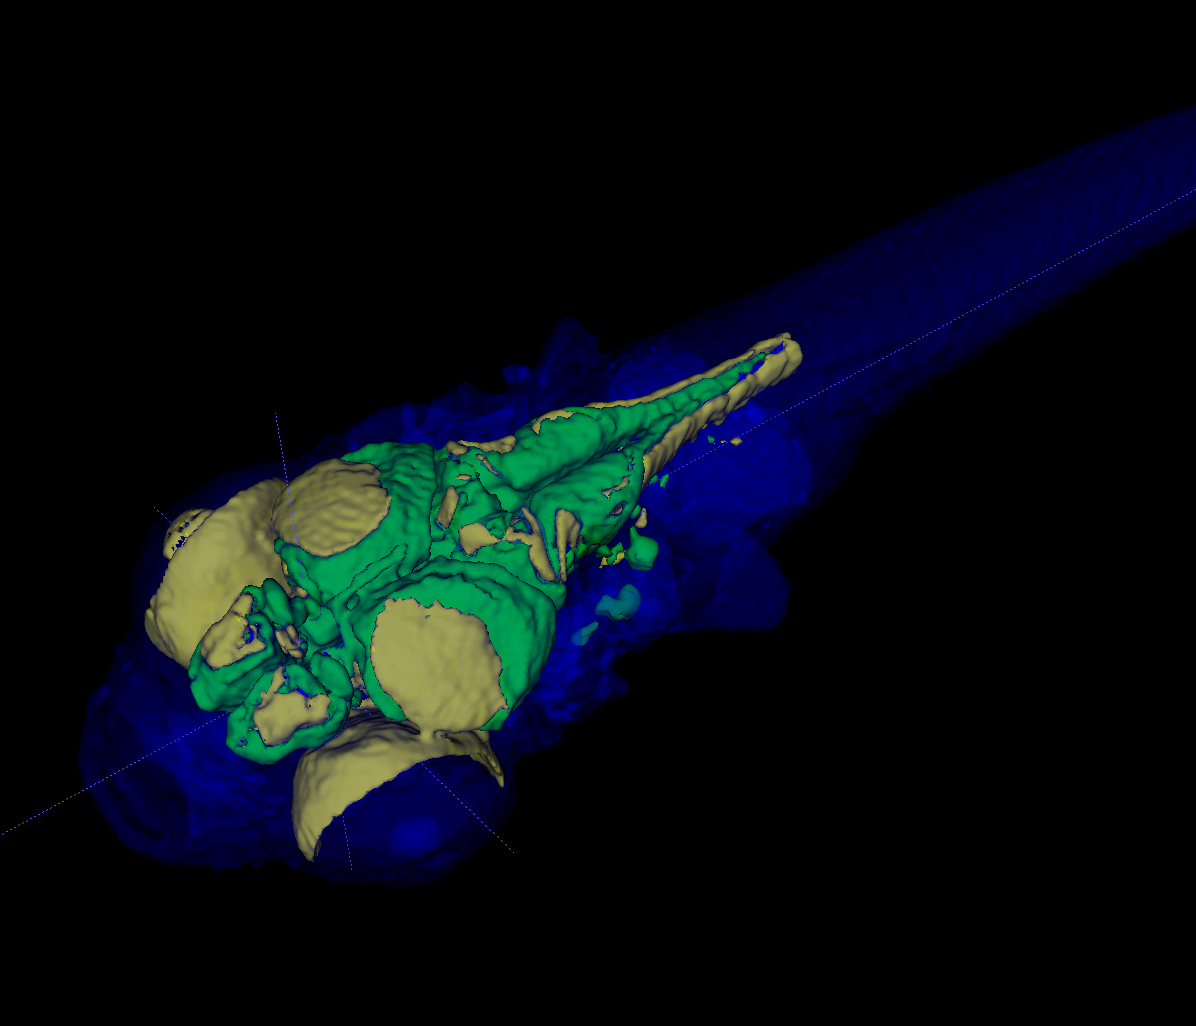
\includegraphics[width=12cm]{Figures/titre.png}\\ \medskip % Picture

\myTime

\begin{tabularx}{\linewidth}{lll}
    Directeur de thèse & Hugues \texsc{Talbot} & Enseignant-chercheur, Centrale Supelec\\
    Directeur de thèse & Jean-Stéphane \texsc{Joly} & Directeur de recherche, INRAE\\
    Rapporteur & Nicolas \texsc{David} & Chargé de recherche, Ecole Polytechnique\\ % Selon son LinkedIn
    Rapporteur & Beatriz \texsc{Marcotegui} & Maitre de recherche, Mines ParisTech\\
    Examinateur & Noémie \texsc{De Crozé} & Ingénieure Recherche Avancée,\newline L'Oréal Recherche et Innovation\\ % Selon la thèse de diane
    Examinateur & Karima Kissa & CSO, Azelead
\end{tabularx}

\vfill

\end{center}
\end{addmargin}

\end{titlepage} % Main title page

% Back of the title page

\thispagestyle{empty}

\hfill

\vfill

%\noindent\myName: \textit{\myTitle,} \mySubtitle, %\myDegree, 
%\textcopyright\ \myTime

% You may wish to do something with the back of the title page, such as including your supervisors, location or time frame of the work. Below is an example of doing so although you may want to tweak it to your liking.

%\bigskip

%\noindent\spacedlowsmallcaps{Supervisors}: \\
%\myProf \\
%\myOtherProf \\ 
%\mySupervisor

%\medskip \\

%\noindent\spacedlowsmallcaps{Location}: \\
%\myLocation

%\medskip \\

%\noindent\spacedlowsmallcaps{Time Frame}: \\
%\myTime
 % Back of the title page

%\cleardoublepage% Dedication

\thispagestyle{empty}
\refstepcounter{dummy}

\pdfbookmark[1]{Dedication}{Dedication} % Bookmark name visible in a PDF viewer

\vspace*{3cm}

\begin{center}
\emph{Ohana} means family. \\
Family means nobody gets left behind, or forgotten. \\ \medskip
--- Lilo \& Stitch    
\end{center}

\medskip

\begin{center}
Dedicated to the loving memory of Rudolf Miede. \\ \smallskip
1939\,--\,2005
\end{center} % Dedication page

%\cleardoublepage\include{FrontBackMatter/Foreword} % Uncomment and create a Foreword.tex to include a foreword

\cleardoublepage% Abstract

%\renewcommand{\abstractname}{Abstract} % Uncomment to change the name of the abstract

\pdfbookmark[1]{Abstract}{Abstract} % Bookmark name visible in a PDF viewer

\begingroup
\let\clearpage\relax
\let\cleardoublepage\relax
\let\cleardoublepage\relax

\chapter*{Abstract}
Short summary of the contents\dots a great guide by 
Kent Beck how to write good abstracts can be found here:  
\begin{center}
\url{https://plg.uwaterloo.ca/~migod/research/beckOOPSLA.html}
\end{center}

\endgroup			

\vfill % Abstract page

\cleardoublepage% Publications - a page listing research articles written using content in the thesis

\pdfbookmark[1]{Publications}{Publications} % Bookmark name visible in a PDF viewer

\chapter*{Publications} % Publications page text

\bibentry{bouffard_2018}
%\bibentry{lempereur_2020}

%\emph{Attention}: This requires a separate run of \texttt{bibtex} for your \texttt{refsection}, \eg, \texttt{ClassicThesis1-blx} for this file. You might also use \texttt{biber} as the backend for \texttt{biblatex}. See also \url{http://tex.stackexchange.com/questions/128196/problem-with-refsection}. % Publications from the thesis page

\cleardoublepage% Acknowledgements

\pdfbookmark[1]{Remerciements}{Remerciements} % Bookmark name visible in a PDF viewer

\begingroup

\let\clearpage\relax
\let\cleardoublepage\relax
\let\cleardoublepage\relax

\chapter*{Remerciements}

Je tiens tout d'abord à remercier Noémie de Crozé et Karima ? qui ont accepté de faire partie de mon jury, ainsi que Nicolas David et Beatriz Marcotegui pour avoir pris le temps de rapporter mon manuscrit de thèse.

\endgroup % Acknowledgements page

\pagestyle{scrheadings} % Show chapter titles as headings

\cleardoublepage% Table of Contents - List of Tables/Figures/Listings and Acronyms

\refstepcounter{dummy}

\pdfbookmark[1]{\contentsname}{tableofcontents} % Bookmark name visible in a PDF viewer

\setcounter{tocdepth}{2} % Depth of sections to include in the table of contents - currently up to subsections

\setcounter{secnumdepth}{3} % Depth of sections to number in the text itself - currently up to subsubsections

\manualmark
%\markboth{\spacedlowsmallcaps{\contentsname}}{\spacedlowsmallcaps{\contentsname}}
\tableofcontents 
\automark[section]{chapter}
\renewcommand{\chaptermark}[1]{\markboth{\spacedlowsmallcaps{#1}}{\spacedlowsmallcaps{#1}}}
\renewcommand{\sectionmark}[1]{\markright{\thesection\enspace\spacedlowsmallcaps{#1}}}

\clearpage

\begingroup 
\let\clearpage\relax
\let\cleardoublepage\relax
\let\cleardoublepage\relax

%----------------------------------------------------------------------------------------
%	List of Figures
%----------------------------------------------------------------------------------------

%\refstepcounter{dummy}
%%\addcontentsline{toc}{chapter}{\listfigurename} % Uncomment if you would like the list of figures to appear in the table of contents
%\pdfbookmark[1]{\listfigurename}{lof} % Bookmark name visible in a PDF viewer

%\listoffigures

%\vspace{8ex}
%\newpage

%----------------------------------------------------------------------------------------
%	List of Tables
%----------------------------------------------------------------------------------------

%\refstepcounter{dummy}
%%\addcontentsline{toc}{chapter}{\listtablename} % Uncomment if you would like the list of tables to appear in the table of contents
%\pdfbookmark[1]{\listtablename}{lot} % Bookmark name visible in a PDF viewer

%\listoftables
        
%\vspace{8ex}
%\newpage
    
%----------------------------------------------------------------------------------------
%	List of Listings
%---------------------------------------------------------------------------------------- 

%\refstepcounter{dummy}
%%\addcontentsline{toc}{chapter}{\lstlistlistingname} % Uncomment if you would like the list of listings to appear in the table of contents
%\pdfbookmark[1]{\lstlistlistingname}{lol} % Bookmark name visible in a PDF viewer

%\lstlistoflistings 

%\vspace{8ex}
%\newpage
       
%----------------------------------------------------------------------------------------
%	Acronyms
%----------------------------------------------------------------------------------------

\refstepcounter{dummy}
%\addcontentsline{toc}{chapter}{Acronyms} % Uncomment if you would like the acronyms to appear in the table of contents
\pdfbookmark[1]{Acronyms}{acronyms} % Bookmark name visible in a PDF viewer

\markboth{\spacedlowsmallcaps{Acronyms}}{\spacedlowsmallcaps{Acronyms}}

\chapter*{Acronymes}

\begin{acronym}[UML]
\acro{ADN}{Acide désoxyribonucléique}
\acro{ARN}{Acide ribonucléique}
\acro{dpf}{jours post-fertilisation (de l'anglais days post fertilization}
\acro{hpf}{heures post-fertilisation}
\acro{wpf}{semaines post-fertilisation (de l'anglais week post fertilisation}
\acro{HCS}{\Hcs{} (de l'anglais high content screening)}
\acro{HTI}{\Hti{} (de l'anglais high troughput imaging)}
\acro{HCA}{\Hca{} (de l'anglais high content analysis)}
\acro{EE}{\Ee}
\acro{VAST}{Vertebrate Automated Screening Technology}
\acro{SBDDCC}{\sbddcc}
\acro{SBLC}{\sblc}
\acro{ZBI}{ZeBraInspector}
\end{acronym} 

\endgroup % Contents, list of figures/tables/listings and acronyms

\listoffigures

\cleardoublepage

\pagenumbering{arabic} % Arabic page numbering for thesis content (1, 2, 3, etc)
%\setcounter{page}{90} % Uncomment to manually start the page counter at an arbitrary value (for example if you wish to count the pre-content pages in the page count)

\cleardoublepage % Avoids problems with pdfbookmark

%----------------------------------------------------------------------------------------
%	THESIS CONTENT - CHAPTERS
%----------------------------------------------------------------------------------------

\providecommand{\main}{..}

\documentclass[\main/main.tex]{subfiles}

\begin{document}

\part{Introduction}

\providecommand{\main}{../..}

\documentclass[\main/main.tex]{subfiles}

\begin{document}

\chapter{
    \label{chap:zebra}
    le \pz{}, un modèle idéal pour les \hcss{}
    }

\providecommand{\main}{../../..}
\providecommand{\Figures}{\main/Figures}

\documentclass[\main/main.tex]{subfiles}

\begin{document}
            
\section{Le \pz{}, le second modèle le plus utilisé en laboratoire}

%%
%
Le \pz{} est une espèce de poisson d'eau douce originaire d'Asie et très commune au nord de l'Inde (voir \autoref{fig:model:zebra}).
%
Il appartient à la famille de Cyprinidae, comme la carpe commune.

\begin{figure}[h!]{\textwidth} 
    \centering
       \centering 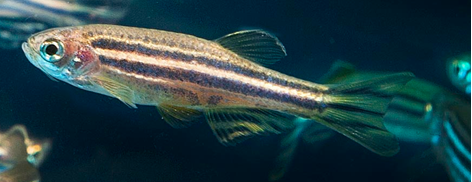
\includegraphics[width=\textwidth]{\Figures/Modeles/adult.png}
       \caption{
            \label{fig:model:zebra}\pz{} adulte. \newline
            Ce poisson d'eau douce est un organisme modèle important pour la communauté scientifique.
            }
\end{figure}

%%
%
Il s'agit du second organisme modèle le plus employé.
%
Presque quatre milles publications ont utilisé le mot "zebrafish" en 2019
selon \href{https://pubmed.ncbi.nlm.nih.gov/?term=zebrafish&sort=pubdate}{PubMed}(voir \autoref{fig:model:pz:stats}).

\begin{figure}[h!]{\textwidth} 
    \centering
       \centering 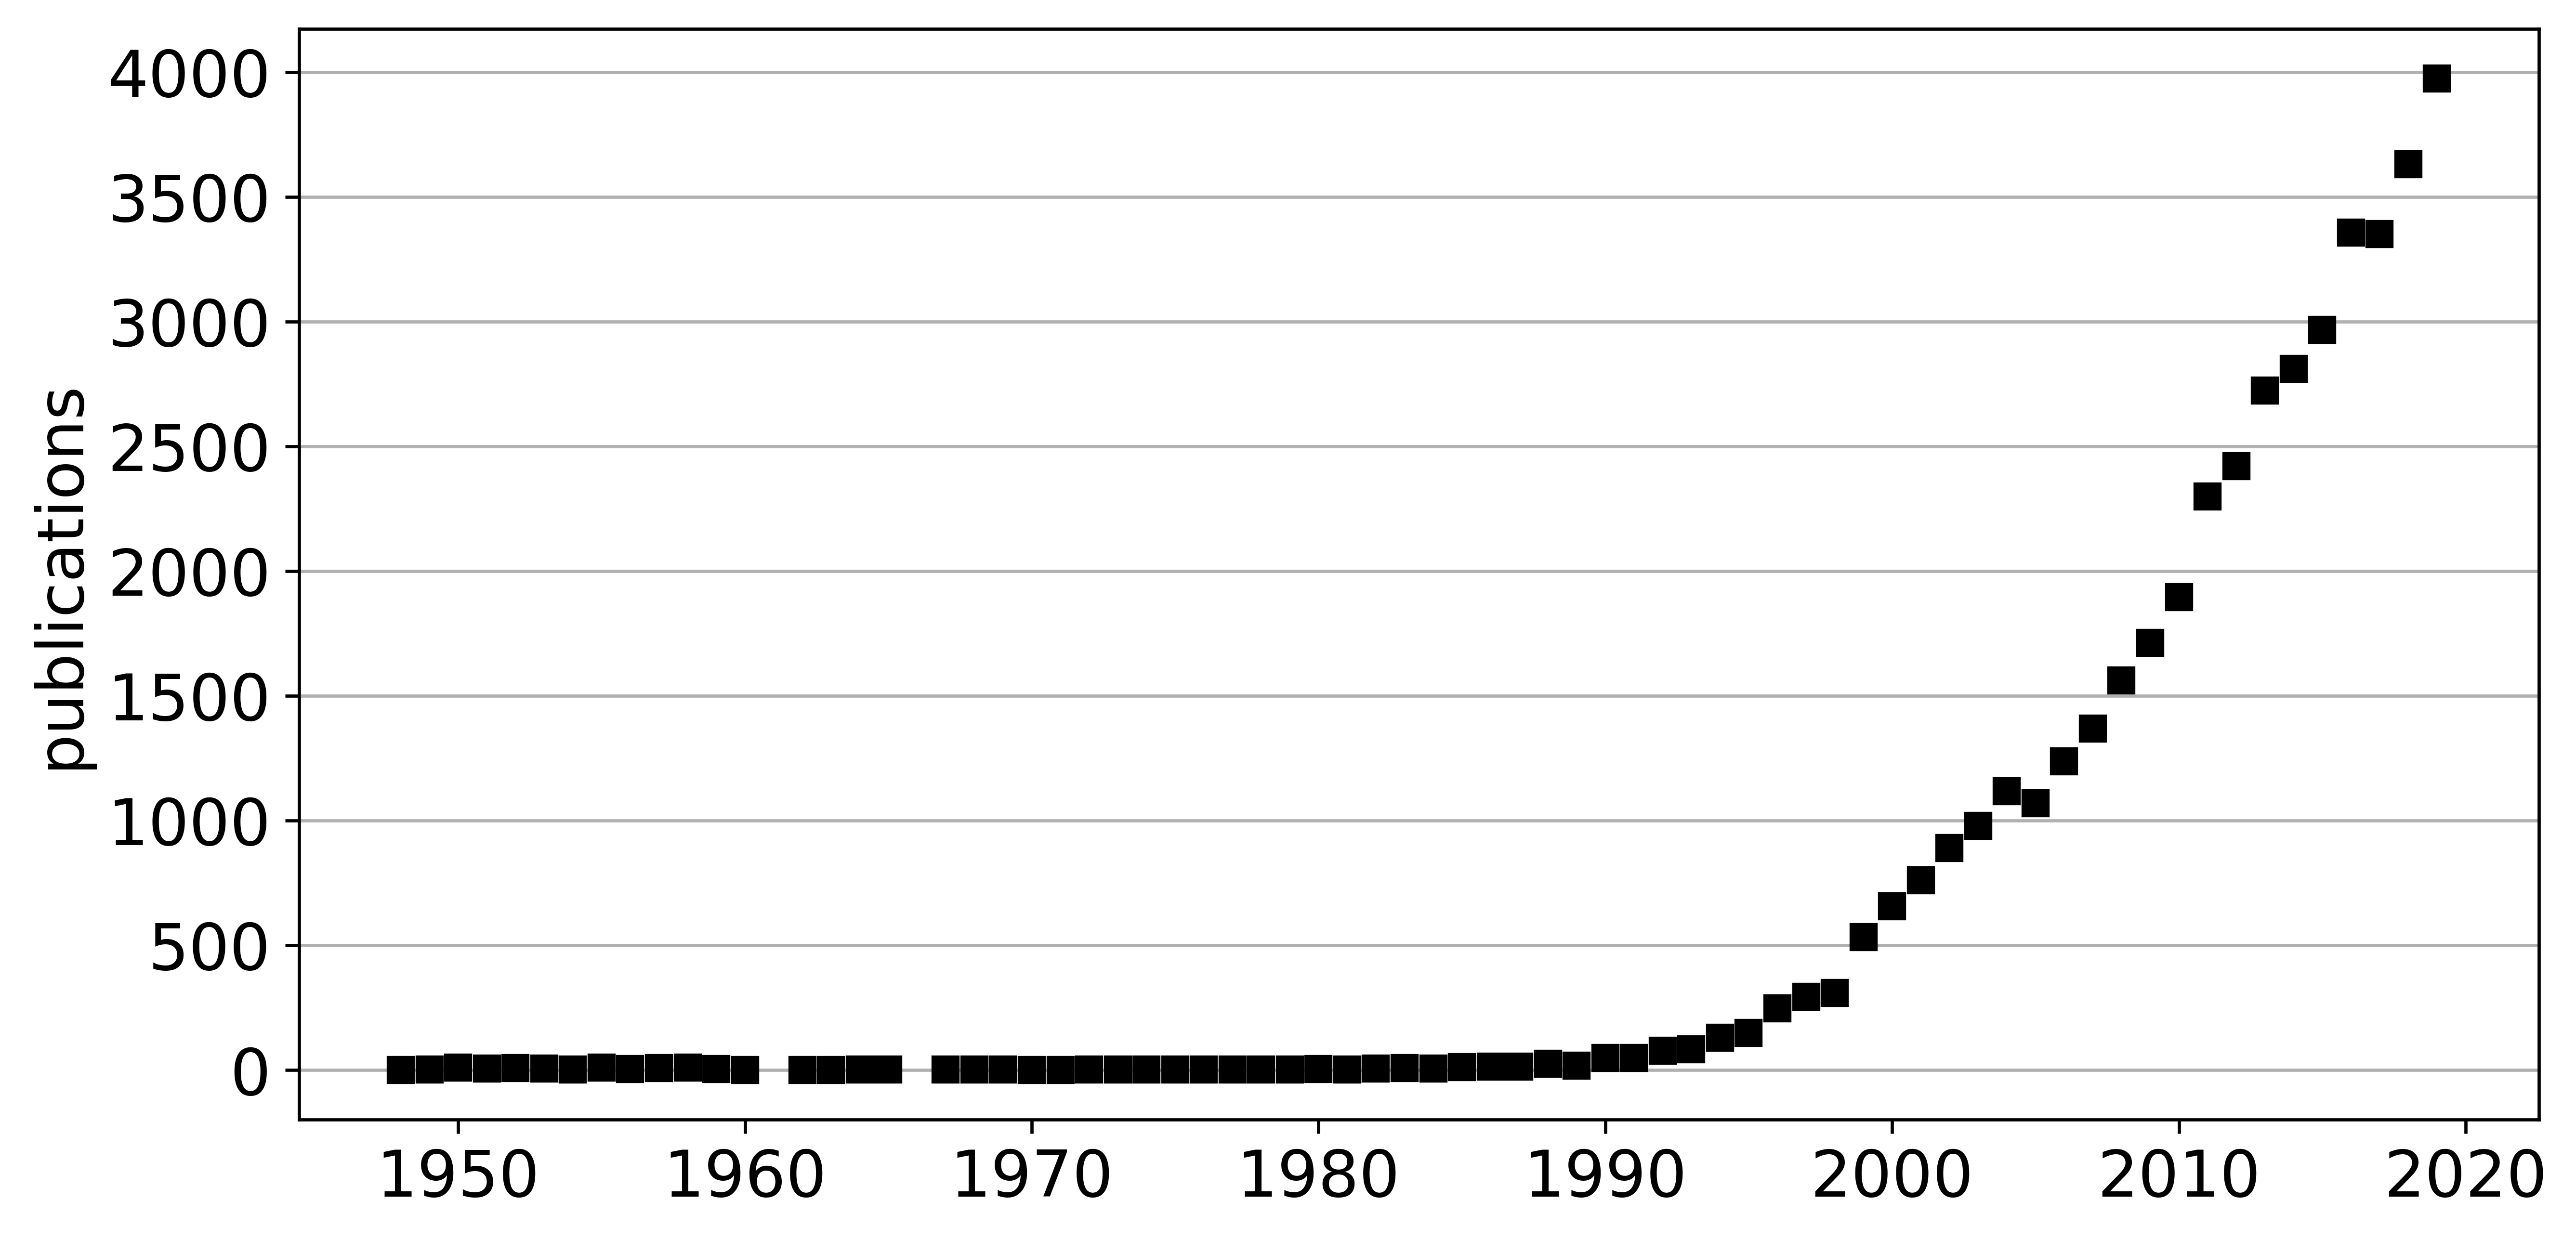
\includegraphics[width=\textwidth]{\Figures/Modeles/publis_zebra.png}
       \caption{
            \label{fig:model:pz:stats}Référencement du terme "zebrafish" au sein de \href{https://pubmed.ncbi.nlm.nih.gov/?term=zebrafish&sort=pubdate}{PubMed}.
            \newline
            Presque 4000 publications en 2019 sur le \pz{}, le second modèle le plus utilisé en laboratoire.
            }
\end{figure}
%
Son utilisation en tant qu'organisme modèle est fréquente pour plusieurs raisons.

    \subsection{Un modèle compact et fertile}
    
%% Petite taille
%
Le \pz{} adulte mesure environ quatre centimètres.
%
Cette petite taille présente plusieurs avantages.

%
Tout d'abord, il est possible d'élever un grand nombre de poissons dans un espace réduit~\cite{avdesh_2012}.
%%
%
Un second avantage de cette petite taille est qu'elle permet de faciliter le transport et les expérimentations avec ce modèle.
%
Il est en effet possible de transporter facilement un grand nombre d'oeufs mais aussi des juvéniles ou des adultes.
%
Cette aspect facilite le partage de lignées mutantes ou transgéniques.
%
\ajout{
La petite taille de cette espèce permet de réduire le coût des expérimentations.
%
Elle permet par exemple d'utiliser moins d'anticorps pour effectuer le marquage \ihc{} d'échantillons entiers ou en réduisant le nombre de champs optiques nécessaires pour la réalisation d'imagerie d'individus entiers.
}
%%
%
La petite taille permet aussi de manipuler facilement un grand nombre d'échantillons en parallèle~\cite{wittbrodt_2014,brion_2012}. Les pipetages à large échelle sont possibles à des stades précoces,
ce qui rend possible l'automatisation de différents traitements~\cite{mandrell_2012,teixid_2019}.

%% Reproduction
Le \pz{} possède une fertilité adaptée aux expériences impliquant un grand nombre d'échantillons.
%
Tout d'abord, la femelle pond les oeufs qui coulent au fond de l'aquarium ce  qui permet de les récupérer aisément. Chaque ponte contient entre 100 et 500 oeufs ce qui permet par exemple facilement d'identifier des combinaisons de mutations dans la descendance d'un animal édité. TPS s'est doté de structures d'élevage qui permettent de caractériser près de 200 poissons en parallèle isolés dans une cage unique dans de bonnes conditions de bien-être (Marie-Elise Schwartz, TPS-AQUA, communication personnelle).  
\ajout{
%
En permettant d'utiliser un plus grand nombre d'échantillons,
la grande quantité d'oeufs obtenus par reproduction permet d'augmenter la significativité statistique des analyses réalisées, ce qui permet de valider des processus biologiques discrets.
}
%
Enfin, dans des conditions optimales d'élevage, le \pz{} devient fertile en environ 3 mois. Cet intervalle entre générations peut être raccourci à 2 mois pour les mâles en utilisant des robots nourrisseurs qui effectuent quatre nourrissages quotidiens, week-end y compris. 


%% Statut légal des eleuthéroembryons (EE) avant 5 jours
Le statut légal du \pz{} aux stades précoces renforce l'intérêt de son utilisation en laboratoire.
%
En effet, une espèce aquatique élevée en laboratoire rentre dans le cadre de la directive européenne n°2010/63/UE seulement à partir des stades larvaires autotrophes environ à 6dpf.
%
Cette définition permet donc de ne pas considérer les stades de développement du \pz{} entre la ponte et 5dpf comme animal de laboratoire nécessitant une autorisation d'expérimenter.
%
\ajout{
L'alevin vésiculé de \pz{} à 5dpf, aussi appelé eleuthéroembryons (EE), est ainsi largement employé en toxicologie.
}
%
De plus, à ces stades, les larves de poissons-zèbre vivantes présentent une forte transparence (voir \autoref{fig:zebra:transparent}),
ce qui permet d'imager des structures non périphériques sans réaliser de coupes~\cite{asokan_2020,chen_2020,hamilton_2016,kioka_2020}.

\begin{figure}[h!]
    \centering
    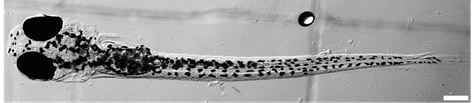
\includegraphics[width=\textwidth]{\Figures/Modeles/larve_5dpf_transparent.png}
    \caption{Vue dorsale d'un EE de \pz{}.\newline
    À des stades de développement précoces, cet organisme modèle est très transparent.
    Il présente néanmoins des mélanocytes pigmentés qui doivent être rendus transparents par un traitement de dépigmentation.
    }
    \label{fig:zebra:transparent}
\end{figure}


%%
%
Malgré tous les avantages présentés ici, l'utilisation du \pz{} en laboratoire serait limité s'il ne possédait pas un grand nombre de ressources dédiées.
%
Nous allons donc maintenant présenter certaines de ces ressources.

    \subsection{De nombreux protocoles expérimentaux sont disponibles chez le \pz{}}
    
%%
%
L'utilisation du \pz{} comme organisme modèle a pris son essor durant les années 1970~\cite{laale_1977}.
%
En 50 ans, ce modèle a ainsi été largement étudié en laboratoire.
%
En particulier, des études ont rapidement essayé de déterminer les conditions optimales nécessaires à une bonne croissance et une reproduction efficace du \pz{} en captivité, dans des conditions de bien-être acceptables~\cite{eaton_1974,eaton_1974a}.
%
De plus, la présence de longue date de cette espèce au sein des laboratoires a permis la mise en place d'au moins 34 fonds génétiques de référence pour les individus sauvages,
permettant d'étudier la diversité des génomes des individus étudiés.
%%
%
Afin d'utiliser au mieux ce modèle, de nombreux outils ont été développés.
%
En particulier, la plupart des techniques permettant de modification de génome ont été adaptées au \pz{}~\cite{auer_2014,irion_2014,foley_2009,bill_2009}.
%
Il est ainsi possible de créer facilement différents types de lignée de \pz{} génétiquement modifiées, que ce soit pour la création de lignées rapportrices~\cite{brion_2012,goldman_2001} ou pour la création de lignées KO ou KI~\cite{liu_2019}.
%%
%
Plusieurs centres de ressources et bases de données ont été créés.
%
Par exemple, le Zebrafish Internation Resource center (ZIRC), situé à Eugen en Oregon, met à disposition de la communauté plus de 43000 lignées.
%
Ce centre de référence permet ainsi d'assurer une meilleure reproductibilité des études
en permettant d'accéder à des poissons ayant un fond génétique déterminé et des insertions ou mutations validées.
%
En plus de ce centre de référence, le Zebrafish Information Network (ZFIN) est une base de données centrée sur le \pz{}.
%
Cette base de données concentre en un unique site l'ensemble des informations utiles pour effectuer des expérimentations sur le \pz{}.
%
Dans ce cadre, un catalogue de protocoles a été mis à disposition pour permettre de faciliter la diffusion des méthodes permettant de travailler avec le \pz{}.

%% Utilisation comme sentinelles environnementales ou dans le cadre de la tératologie
%
Ce modèle est aussi référencé par des institutions gouvernementales pour le développement d'essais toxicologiques.
%
L'OCDE a ainsi émis différents protocoles visant à standardiser son utilisation pour l'étude de la toxicité aiguë pour les embryons~\cite{oecd_2013}. Ces tests peuvent mesurer la toxicité à de courtes expositions durant les stades précoces (embryon et eleutheroembryon)~\cite{oecd_2013a} ou bien étudier  des stades plus tardifs, et par exemple caractériser les défauts de croissance juvénile suivant l'exposition à des molécules toxiques~\cite{oecd_2000}.
%
La directive REACH de l'Union Européenne, qui vise à réglementer les études des risques liés aux substances chimiques, se concentre particulièrement sur l'étude des perturbateurs endocriniens.
%
Dans ce cadre, une méthode de mise en évidence de l'activité endocrine d'une substance chimique sur des EEs de \pz{} est reconnue comme méthode de référence~\cite{europeanchemicalagencyechaandeuropeanfoodsafetyauthorityefsawiththetechnicalsupportofthejointresearchcentrejrc_2018}.

Il ne fait pas de doute que le  pertinence du \pz{} pour détecter d'éventuels effets délétères de molécules chimiques sur les poissons des rivières et même les poissons marins. En revanche, du fait de la distance évolutive avec l'homme, les conclusions tirées d'études sur le \pz{} ne peuvent constituer que de premiers éléments  qui doivent être confirmés par des tests sur d'autres espèces , bien évidemment des mammifères, mais aussi des amphibiens. En cas de caractérisation d'effets toxiques d'une molécule sur les stades précoces, on peut considérer le \pz{} comme un lanceur d'alerte concernant le potentiel tératogénique de cette molécule en particulier. En aucun cas, l'absence d'effet ne peut être une preuve de son inocuité. 
%

    \subsection{De nombreuses applications en recherche biomédicale}

%
Le \pz{} possède 80\% de gènes homologues communs avec l'humain~\cite{howe_2013}. 
Ce taux d'homologie permet d'utiliser le \pz{} pour la modélisation d'un certain nombre de maladies humaines.
En particulier avec l'apparition des dernières méthodes d'édition du génome permettant d'introduire des mutations ponctuelles par réverse transcription ("base editing", ref), il est possible de modéliser les maladies humaines avec précision chez le \pz{}, en introduisant chez le \pz{} des variations à des positions orthologues chez l'humain où se trouvent des variations génomiques pathogènes.
Bien entendu, ces modèles, en particulier du fait de leur capacité à effectuer de la microscopie à haut-contenu et haut-débit contribuent à la compréhension des mécanismes physio\hyp{}pathologiques, du génotype au phénotype, et à éclairer comment une mutation entraîne des effets cellulaires ciblés et parfois discrets sur le long terme , dans le cadre de l'organisme entier.
Ils permettent aussi permettre d'effectuer des études pré-cliniques visant à déterminer des cibles thérapeutiques, voir tester des traitements contre ces maladies~\cite{vaz_2018,pitchai_2019,saleem_2018} en particulier les thérapies innovantes utilisant des cellules souches ou immunitaires, ou des méthodes d'édition du génome. 
%
Une grande diversité de maladies sont abordées, car l'EE et les juvéniles possèdent des organes très similaires à l'humain, même s'ils sont de plus petite taille et considérablement simplifiés. On peut par exemple citer les maladies neurodégénératives~\cite{fontana_2018}, les anomalies du développement~\cite{lovely_2016,sarmah_2016} ou les maladies cardiaques~\cite{brown_2016, walcott_2014}.

\ajout{
La \autoref{table:zebra} résume les divers avantages du modèles \pz{}.
}

\section{Autres modèles animaux pouvant tirer profit des résultats de ma thèse \label{sec:intro:modele}}
\sectionmark{Autres modèles animaux}

Nous allons maintenant présenter trois espèces par ordre croissant de divergence avec le \pz{}: le médaka, le xénope et la souris.

    \subsection{\label{sec:medaka}Le médaka, un modèle complémentaire au \pz{} très utilisé en toxicologie}
    
%
Le médaka est un poisson téléostéen originaire d'Asie du Sud-Est (voir \autoref{fig:medaka}).

\begin{figure}[h!]
    \centering
    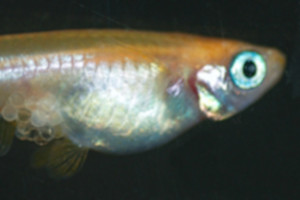
\includegraphics[width = 0.5\textwidth]{\Figures/Modeles/medaka.jpg}
    \caption{
    Femelle médaka portant une grappe d'oeufs située sous son ventre.
    \newline
    Son développement embryonnaire plus long que le \pz{} et sa capacité à résister au froid permet de faciliter l'envoi d'échantillons.
    }
    \label{fig:medaka}
\end{figure}

%
Il est de taille comparable au \pz{} et présente une gestation courte et prolifique.
%
Sa capacité à résister au froid, et son développement embryonnaire, non pas de 48h comme chez le \pz{} mais de l'ordre de dix jours,  facilite son transport, permettant ainsi par exemple pour une plateforme de facilement distribuer des oeufs à d'autres laboratoires.
%
Plusieurs outils de modification du génome ont été mis en place chez \ol{}\cite{kirchmaier_2015, ansai_2017},
ce qui permet la création de lignées rapportrices, de lignées knock-out et de lignées knock-in~\cite{abdelmoneim_2018,jin_2020,Watakabe_2018,qiu_2014,gay_2018}.
%
Enfin, à l'instar du \pz{} avant 120 heures post fertilisation,
le médaka avant 240 heures post-fécondation n'est pas autotrophe.
%
Les embryons et eleutheroembryons ne sont donc pas dans le périmètre de la directive 2010/63/EU de l'Union Européenne.
%
Ainsi, ces stades ne font pas l'objet de demande d'expérimentation animale avant tout projet étant susceptible d 'induire une douleur.

%
C'est aussi un poisson très résistant, qui possède un génome plus compact que le \pz{} , est très distant évolutivement de ce dernier (plus de distance qu'entre le poulet et l'homme), de très bons taux en édition du génome du fait de la possibilité de refroidir l'oeuf. Il possède aussi de nombreuses sous espèces ou espèces soeurs , dont certaines sont maaines, ce qui permet de très intéressantes études comparées.
%
On retrouve ainsi les premières publications utilisant \ol{} dès 1921~\cite{aida_1921}.
%
Son utilisation dans le cadre de publications scientifiques reste assez faible, avec en moyenne deux cents publications annuelles référencées par PubMed(voir \autoref{fig:model:oz:stats}).
%
Mais il est par exemple utilisé dans l'étude du système reproducteur~\cite{gay_2018,herberg_2018} ou
en toxicologie~\cite{carvan_2007,bertotto_2019,cleary_2019,powe_2018}.
%
En particulier, son utilisation dans l'étude des perturbateurs endocriniens a été l'objet d'un protocole de l'OCDE~\cite{oecd_2009}, en faisant un organisme de choix dans l'étude de l'activité endocrine d'une molécule~\cite{chen_2018,dang_2019,spirhanzlova_2016}.

\begin{figure}[h!]{\textwidth} 
    \centering
       \centering 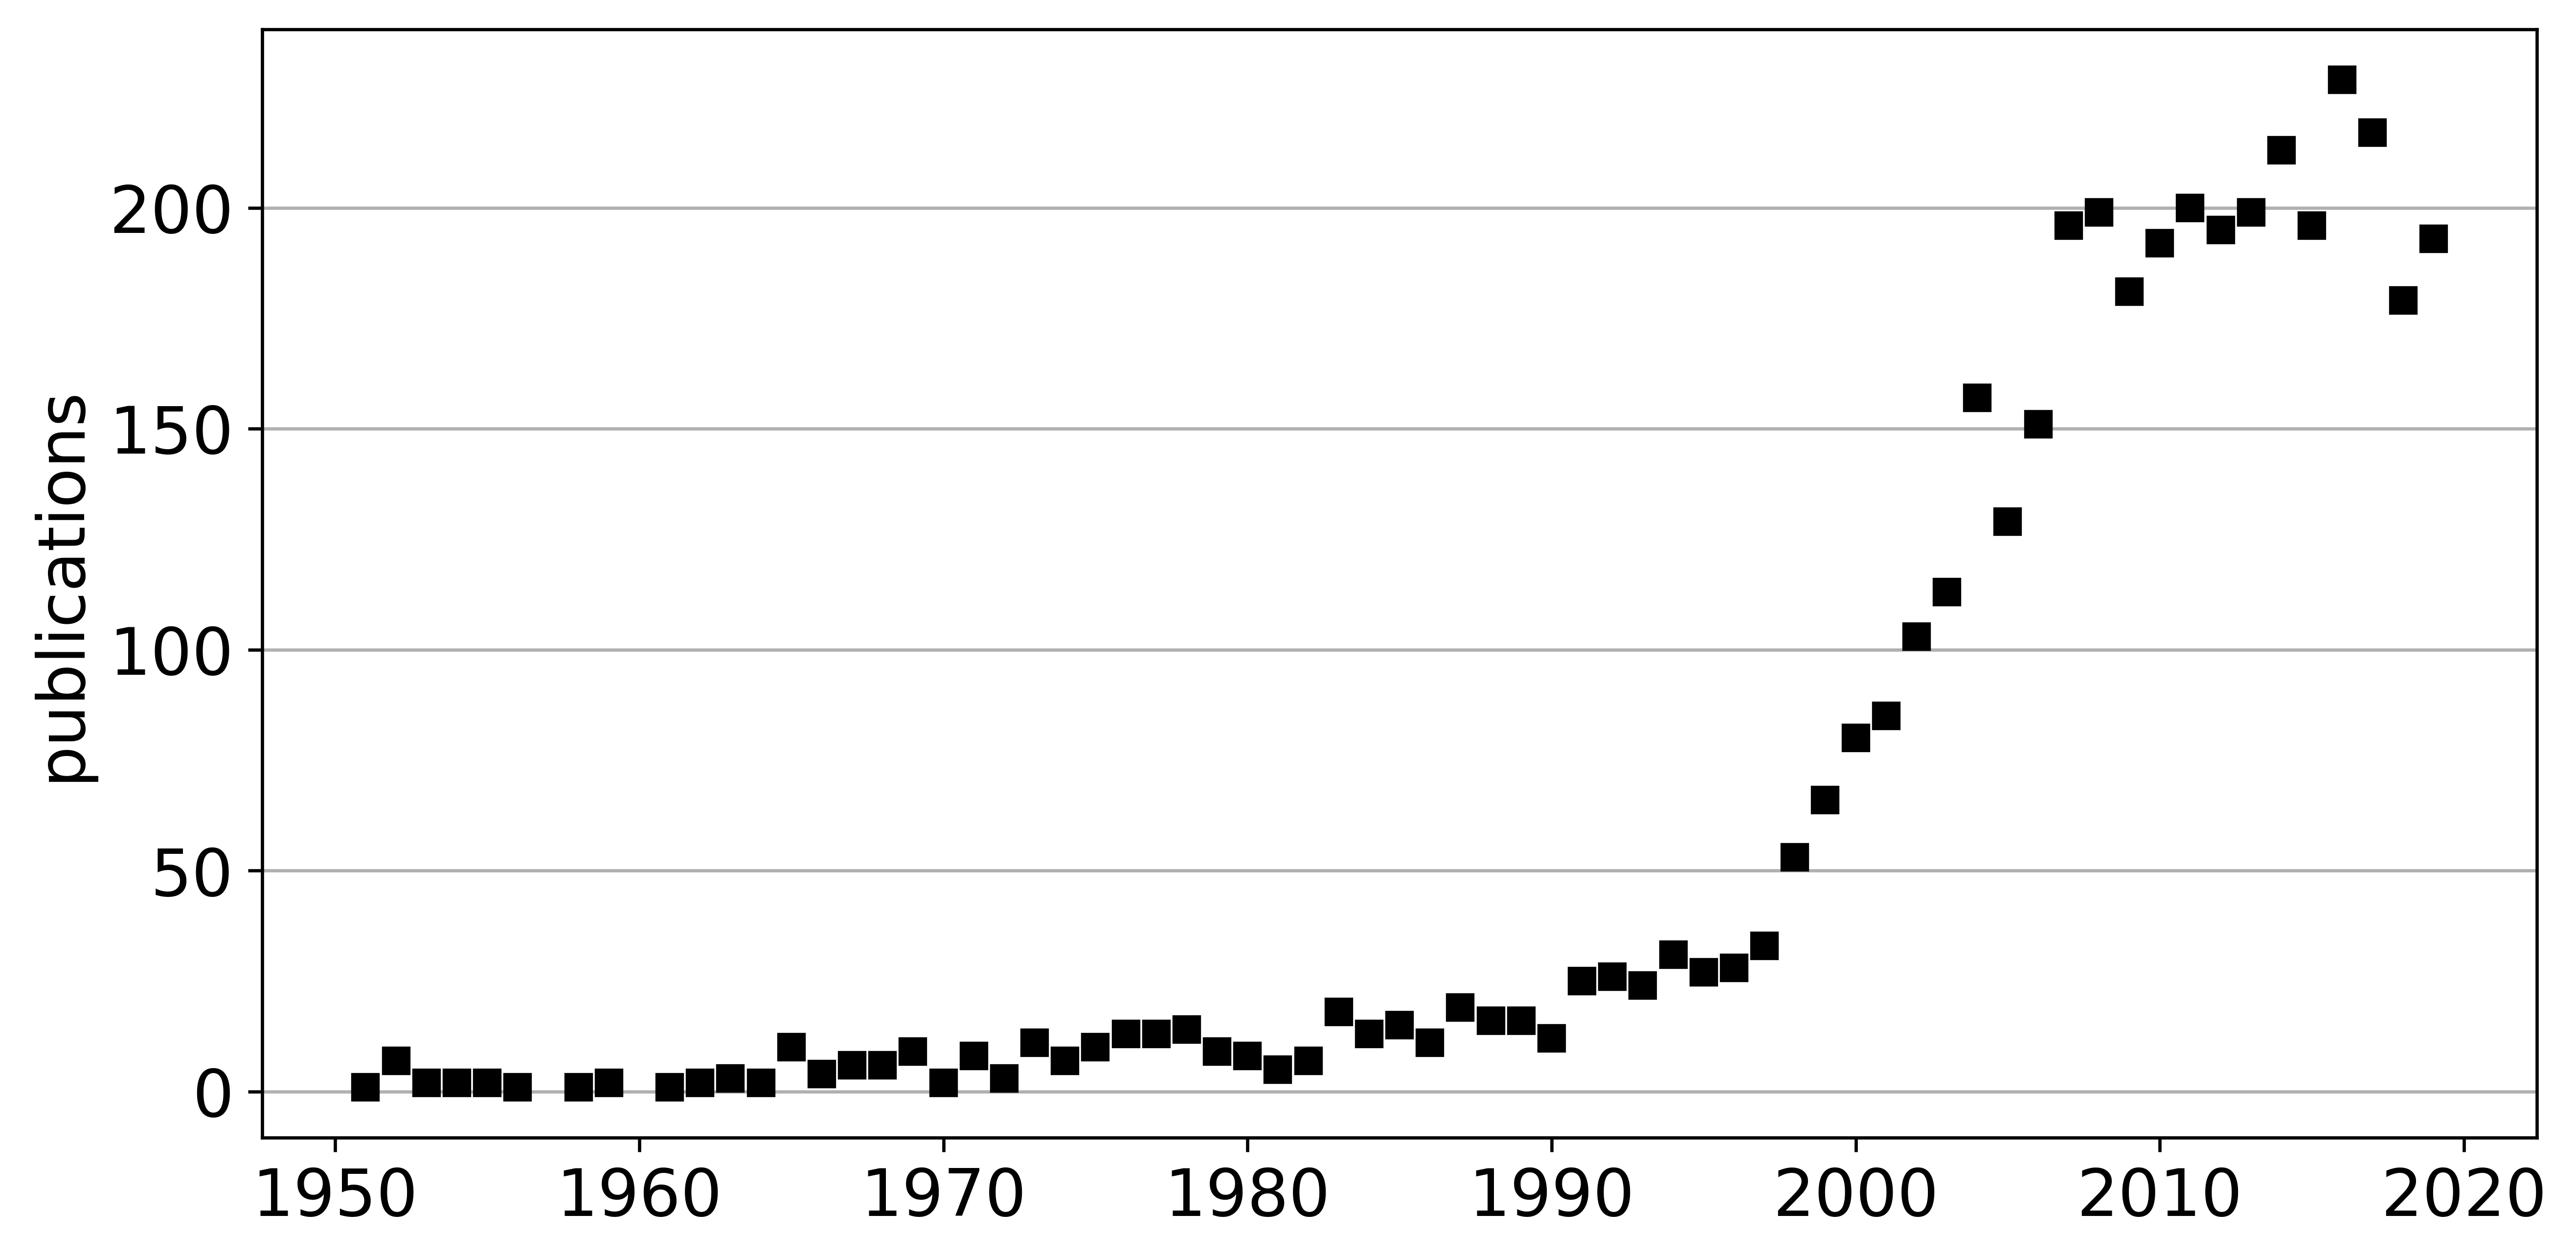
\includegraphics[width=\textwidth]{\Figures/Modeles/publis_medaka.png}
       \caption{
            \label{fig:model:oz:stats}Référencement du terme "medaka" au sein de \href{https://pubmed.ncbi.nlm.nih.gov/?term=medaka&sort=pubdate}{PubMed}.\newline
            Le médaka est un modèle complémentaire au \pz{}, surtout utilisé en toxicologie. La communauté de chercheur travaillant sur le médaka reste de taille beaucoup plus restreinte que celle travaillant sur le \pz{}.
            }
\end{figure}

Les premières utilisations du médaka dans le cadre de \hcs{} sont référencées dès les années 1980~\cite{cameron_1985,Hatanaka_1982}.
%
Cependant, il s'agit d'un organisme rarement référencé pour le \hcs{} par imagerie~\cite{gierten_2020,genest_2019}.

%
Il est pourtant possible d'utiliser un système d'imagerie développé sur le \pz{}
en effectuant peu de modifications pour le faire fonctionner sur le médaka.

    \subsection{Le xénope, un modèle de référence en biologie du développement}

%
\xl{} est une espèce d'amphibiens originaire respectivement d'Afrique de l'ouest et d'Afrique australe (voir \autoref{fig:model:xl}).
%
Bien qu'une femelle ne puisse être stimulée pour la reproduction que tous les trois mois,
sa capacité à produire jusqu'à 4000 oeufs par ponte permet d'avoir rapidement un grand nombre d'échantillons.
%
Elle est en particulier connue du grand public pour être la base d'un des premiers procédés de détection de grossesse chez l'humain dans les années 1950~\cite{hobson_1958,Dittebrandt_1949,polack_1949}
et pour avoir servi de modèle pour le clonage , ce qui a été récemment récompensé en incluant aux côtés d'autres chercheurs \textsc{John Gurdon}  dans un prix Nobel attribué au clonage.

\begin{figure}[h!]{\textwidth} 
    \centering
       \centering 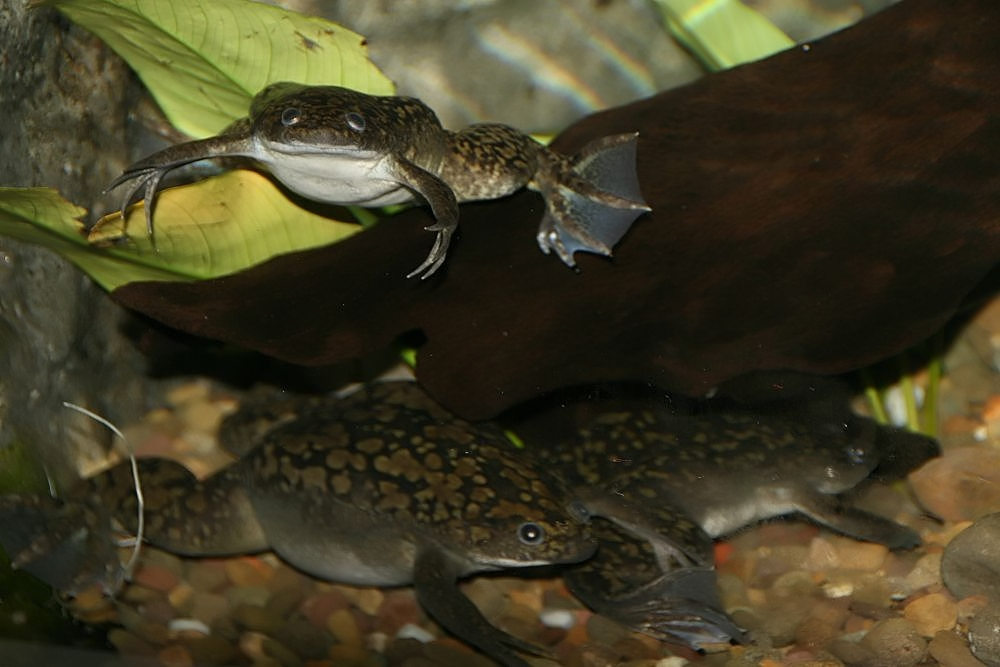
\includegraphics[width=0.75\textwidth]{\Figures/Modeles/xenope.jpg}
       \caption{
            \label{fig:model:xl}
            Xénopes adultes.
            \newline
            C'est un modèle utilisé de longue date en embryologie.
            Ses ovocytes sont aussi utilisés pour exprimer des protéines.
            De plus, sa métamorphose étant contrôlée par des hormones thyroïdienne, il s'agit d'un modèle de choix pour l'étude des perturbateurs endocriniens.
            \newline
            Photographie prise par David J. Stang et mise à disposition sour licence  Creative Commons Attribution-Share Alike 4.0 International
            }
\end{figure}


%%
%
Il s'agit d'un organisme modèle donc établi de très longue date dans la communauté scientifique.
%
Les premières publications scientifiques l'utilisant date de 1930~\cite{edgeworth_1930},
et plus de 1000 publications y faisaient dès l'an 2000.
%
Son utilisation est cependant en baisse depuis 2010. (voir \autoref{fig:model:xl:stats}).
%

\begin{figure}[h!]{\textwidth} 
    \centering
       \centering 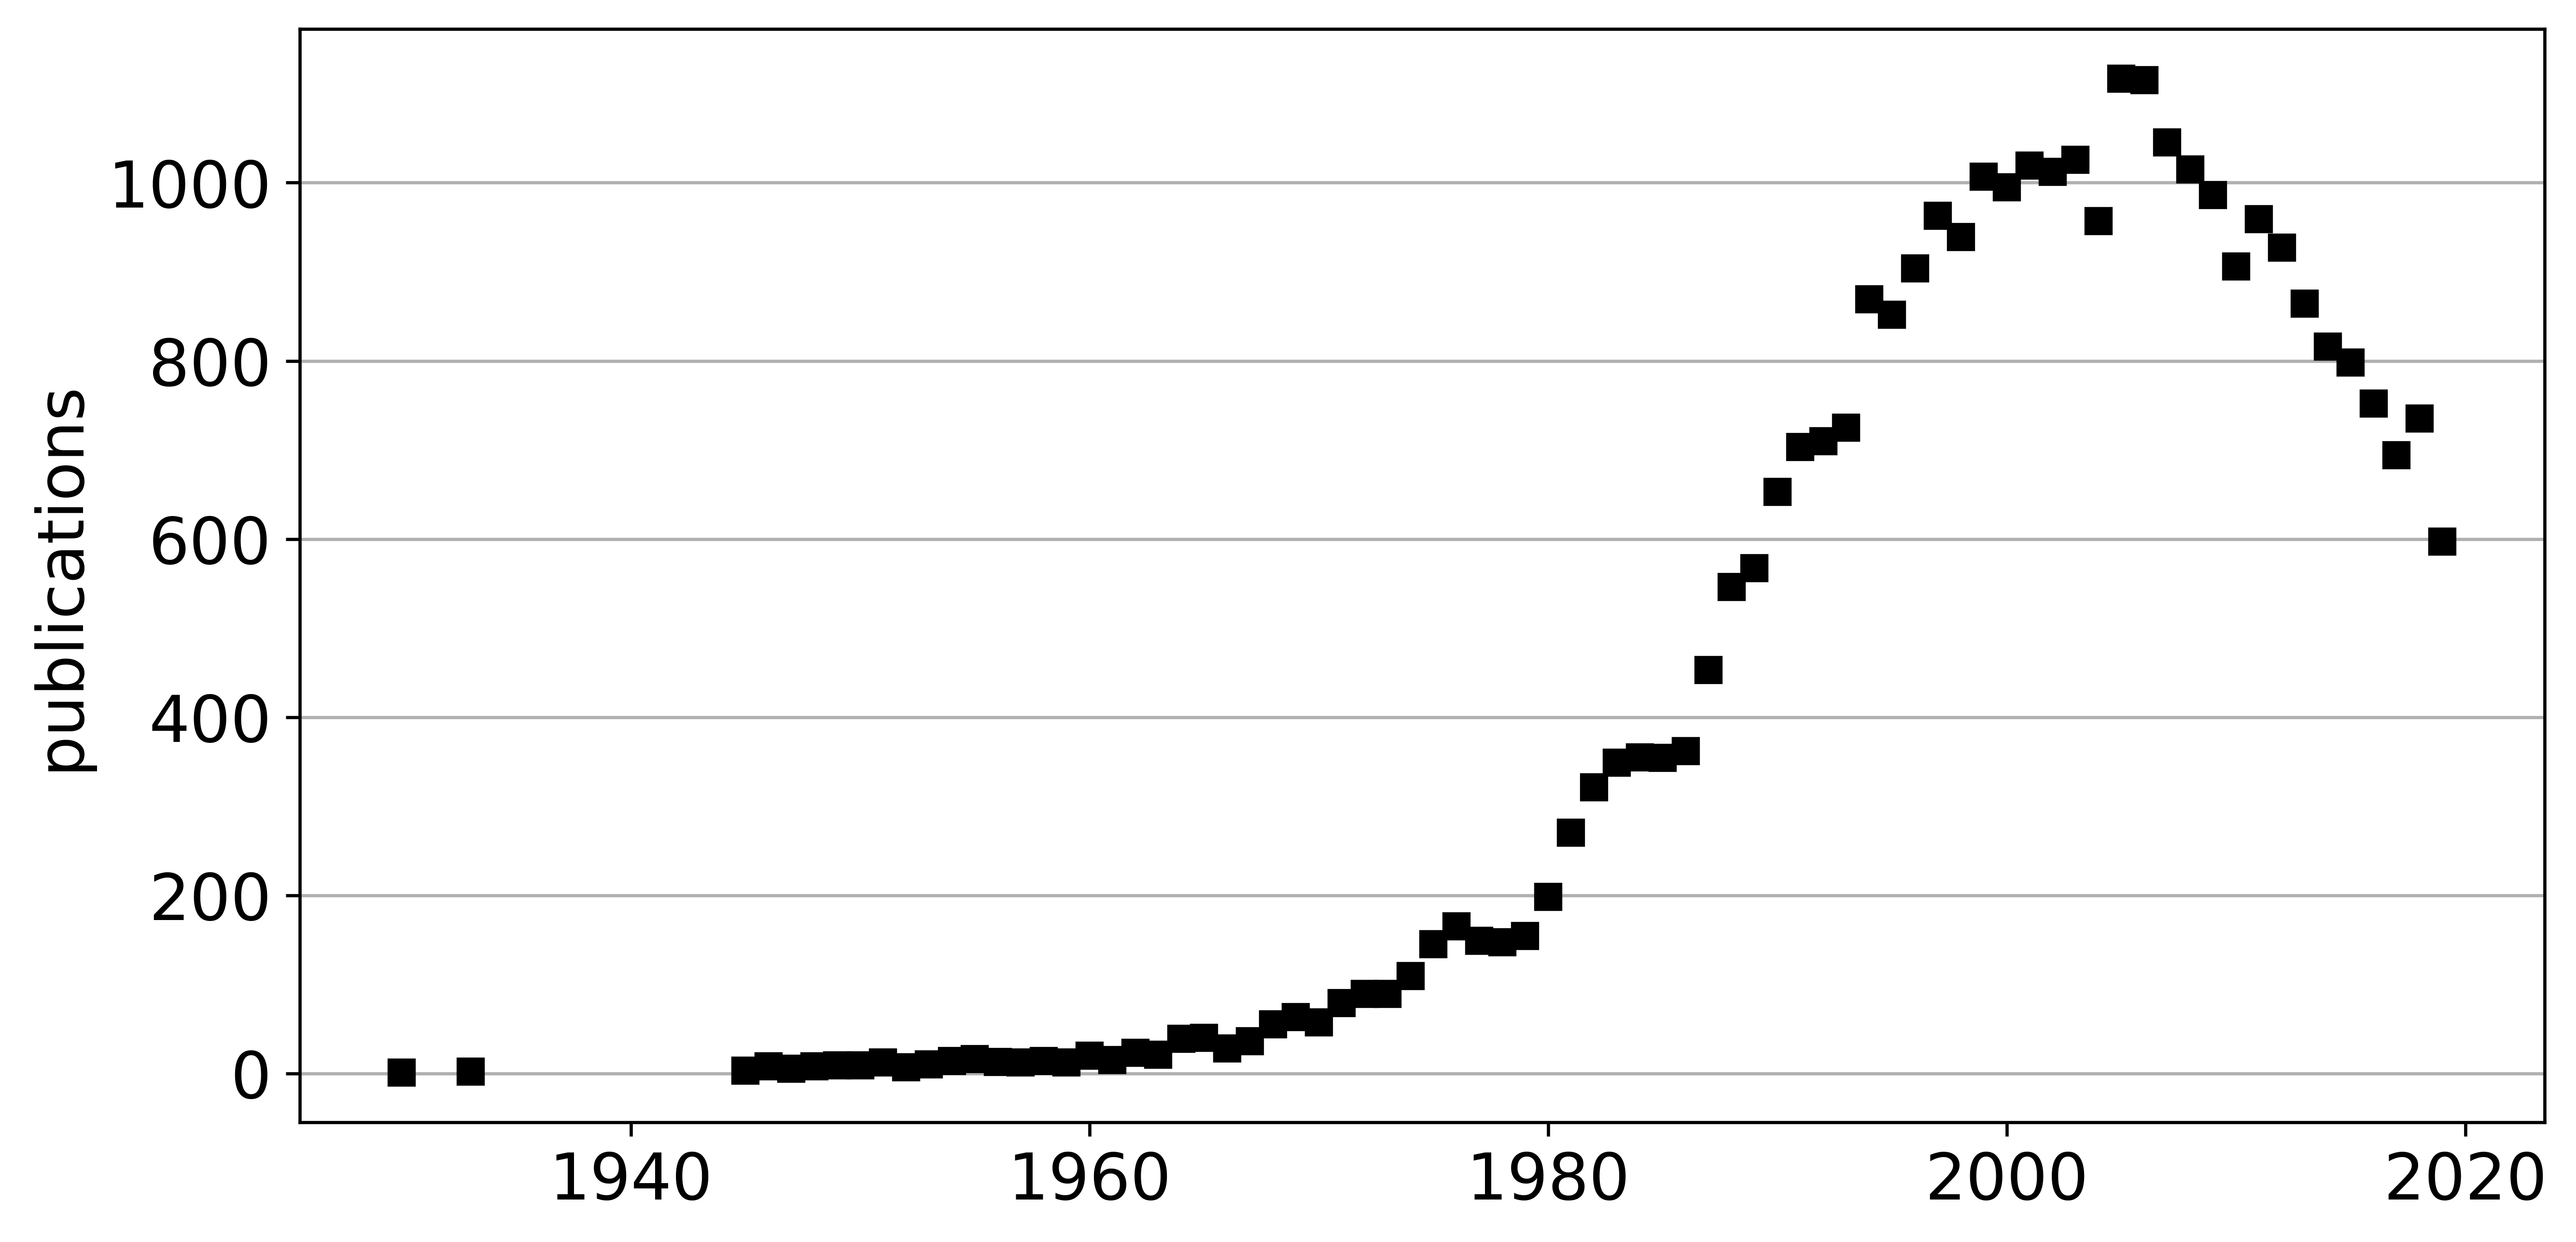
\includegraphics[width=\textwidth]{\Figures/Modeles/publis_xenopus.png}
       \caption{
            \label{fig:model:xl:stats}Référencement des termes "xenopus laevis" au sein de \href{https://pubmed.ncbi.nlm.nih.gov/?term=xenopus+laevis&sort=pubdate}{PubMed}.\newline
            Le xénope est un modèle historiquement très utilisé qui reste encore important pour la communauté scientifique même si le nombre de publications est en baisse.
            }
\end{figure}

%%
%
Le xénope est un modèle d'intérêt pour plusieurs domaines.
%
Il s'agit par exemple d'un modèle de référence dans l'étude du système visuel~\cite{viet_2020,Rahman_2020,kha_2020},
en particulier grâce à sa capacité de régénération de la lentille de l'oeil après ablation de cette lentille~\cite{henry_2019}.
%
Le passage de l'état de têtard à l'état juvénile, appelé métamorphose, est contrôlé chez \xl{} par des hormones thyroïdiennes~\cite{brown_1996,furlow_2006}.
%
Cette particularité rend ce modèle particulièrement intéressant dans l'étude des perturbateurs thyroïdiens~\cite{li_2019,li_2019a,Couderq_2020}.
%
Enfin, \xl{} ne développe que peu de cancers spontanés~\cite{ruben_2007} mais il est possible d'induire la formation de tumeurs. Ces caractéristiques en font un modèle de choix aussi bien dans l'étude de la réponse immunitaire anti-tumorale que dans le développement des cancers~\cite{hardwick_2015}.
%
 Ces dernières années, le développement de méthodes de transgénèse chez \xl{}~\cite{tandon_2017} a permis la mise en place rapide de lignées rapportrices ou de lignées permettant l'étude de mutations responsables de maladies humaines.

    \subsection{La souris, un modèle omniprésent en neuroscience}

%%
La souris est l'organisme vertébré le plus étudié en laboratoire.
%
Son utilisation  est décrite dès le dix-septième siècle.
%
Plus de 80000 publications référençaient ce modèle en 2019 (voir \autoref{fig:model:mm:stats}).

\begin{figure}[h!]{\textwidth} 
    \centering
       \centering 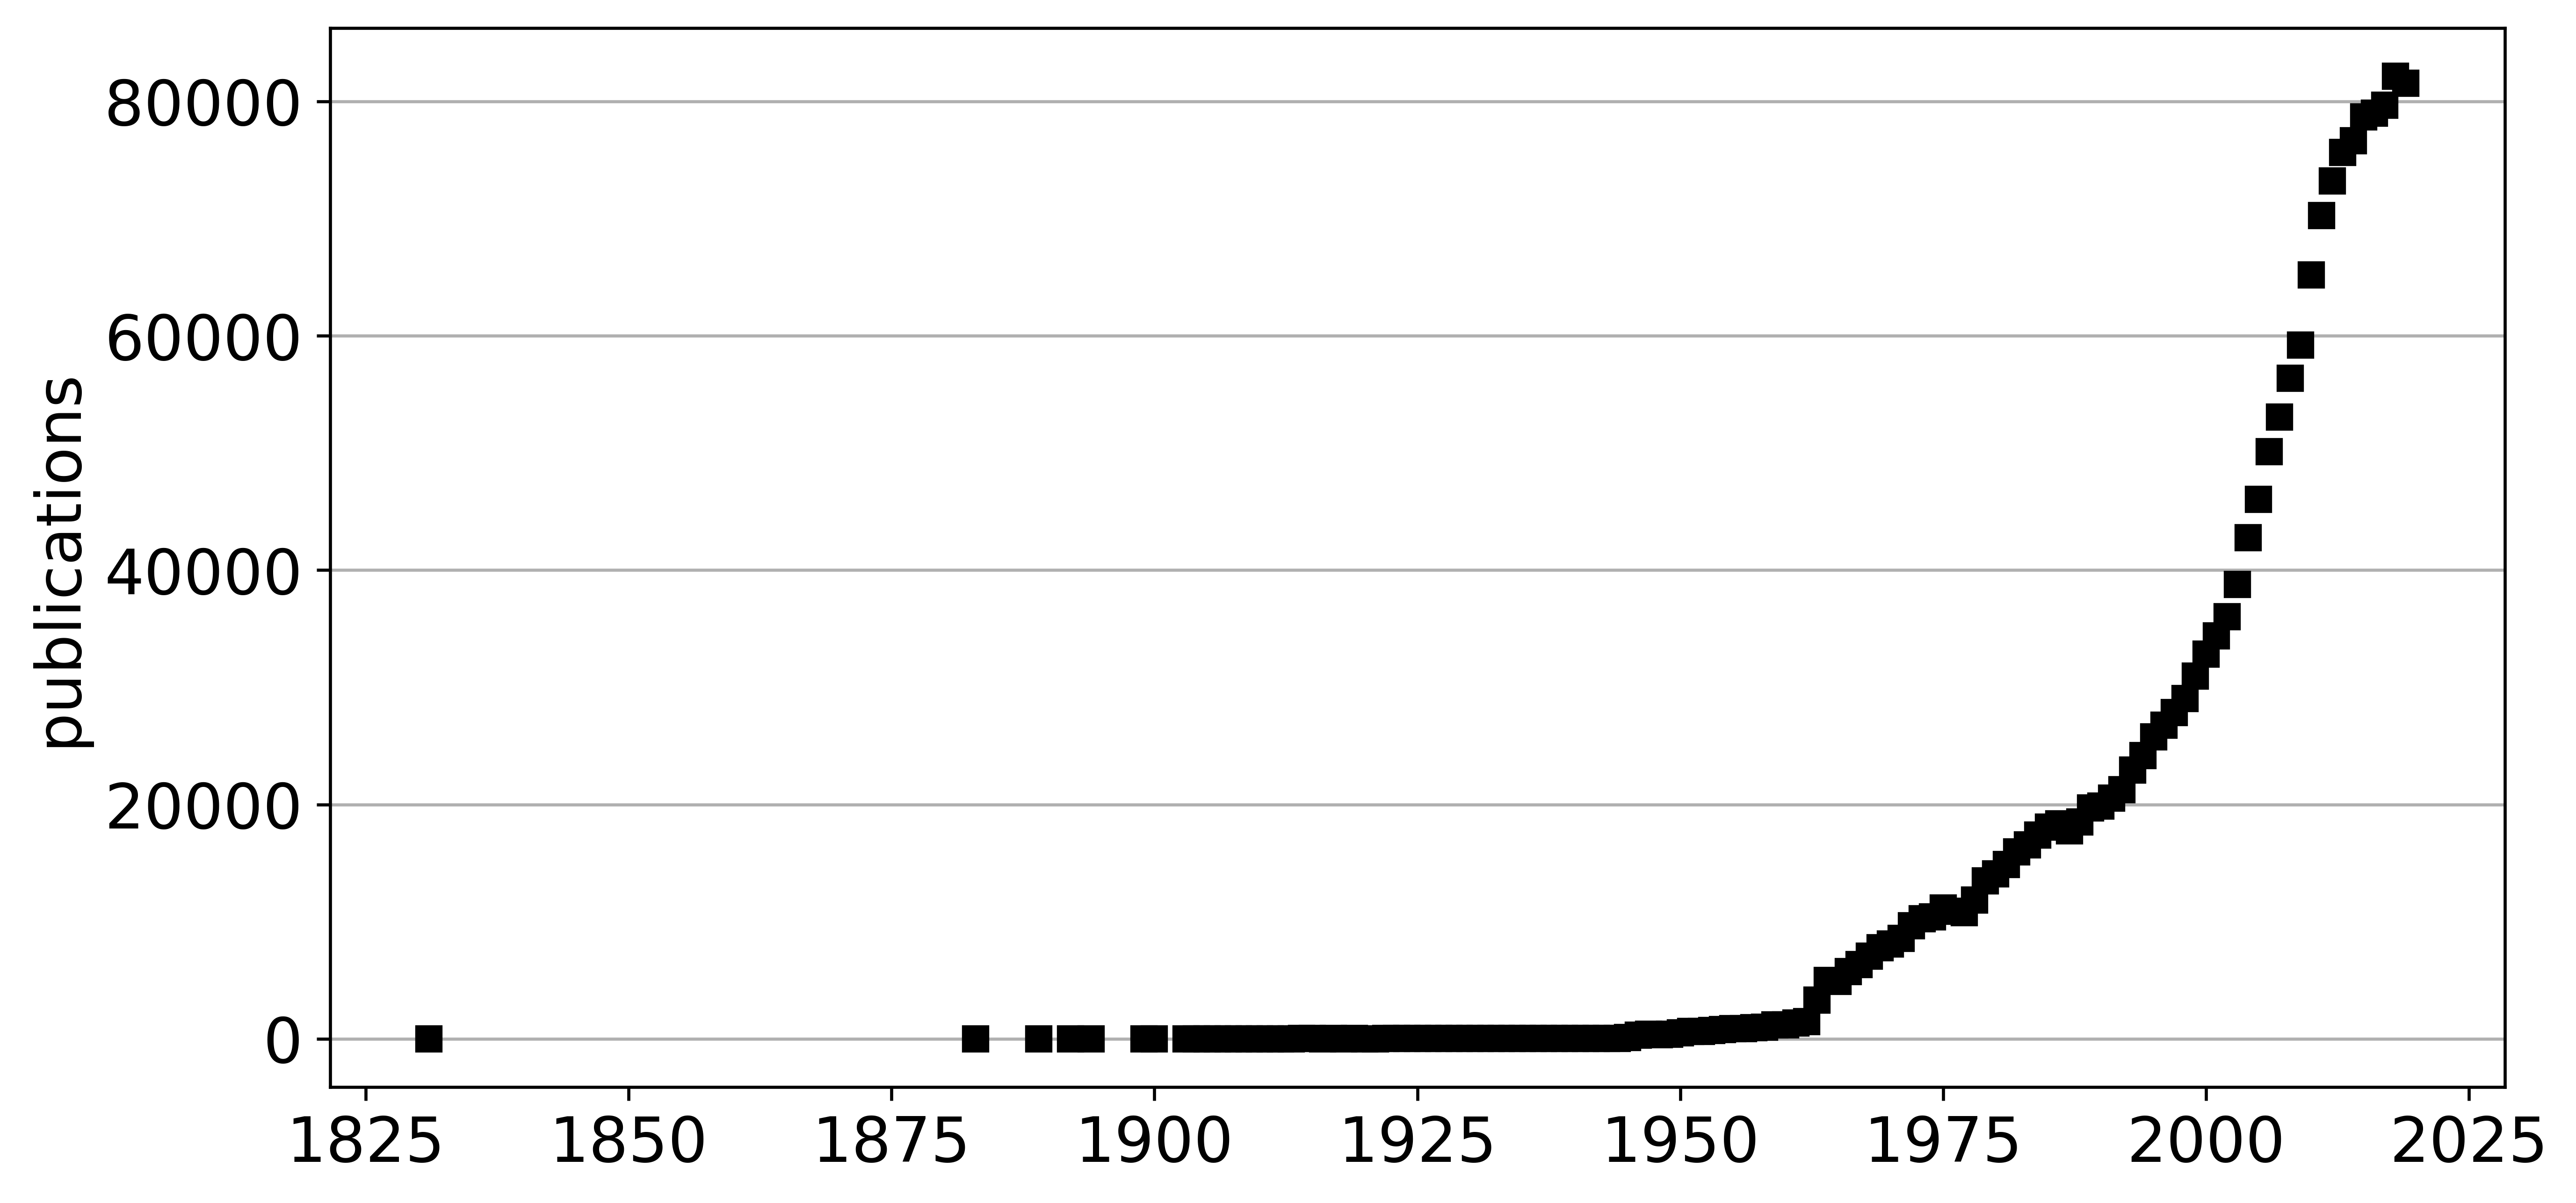
\includegraphics[width=\textwidth]{\Figures/Modeles/publis_mus.png}
       \caption{
            \label{fig:model:mm:stats}Référencement des termes "mus musculus" au sein de \href{https://pubmed.ncbi.nlm.nih.gov/?term=mus+musculus&sort=pubdate}{PubMed}.\newline
            La souris est incontestablement le modèle le plus utilisé par les chercheurs.
            }
\end{figure}

%
Les outils permettant la modification de son génome sont largement développés~\cite{lanigan_2020}.
%
Il est donc possible de modifier le génome de souris pour pouvoir utiliser ce modèle comme outil d'étude de pathologie humaine.
%
Par exemple, la souris est régulièrement utilisée pour étudier diverses maladies neurodégénératives,
comme la maladie d'Alzheimer~\cite{han_2020,thadathil_2020,shin_2020},
la sclérose latérale amyotropique~\cite{Ahmed_2020,konopka_2020,mcleod_2020}
ou la maladie de Huntington~\cite{deng_2020,dridi_2020,pfister_2020}.

%%

\end{document}

\providecommand{\main}{../../..}

\documentclass[\main/main.tex]{subfiles}

\begin{document}
            
\section{Imagerie du \pz{}}

\label{sec:imagerie}

Afin d'être par exemple en mesure de détecter les déformations induites par l'exposition d'un \pz{} à un polluant,
ou d'analyser le patron de fluorescence d'une lignée rapportrice,
il est nécessaire d'adapter différents systèmes d'imagerie aux \pz{}.
%
Nous allons donc présenter différents systèmes d'imageries en fluorescence utilisés chez le \pz{}.

    \subsection{Microscopie}
    
%% Epifluo
La manière la plus simple d'effectuer une imagerie en fluorescence implique l'épifluorescence.
Ceci consiste à émettre un faisceaux lumineux par le moyen d'une source lumineuse avec un spectre variant de l'infrarouge jusqu'à l'ultraviolet.
%
La sélection de la longueur d'onde désirée pour l'observation se fait simplement par le choix d'un filtre.
%
La simplicité, la rapidité et le faible coût de cette approche la rends particulièrement répandue dans les laboratoires, alors qu'elle présente plusieurs limitations.
%
Son défaut principal est sa forte profondeur de champs.
%
Quelque soit la position du plan focal, le détecteur recevra des photons d'autres positions en Z, ce qui limite fortement la résolution de l'image, même si des post-traitements dits de déconvolution sont effectués.


%% confocal
%
La microscopie confocale par balayage laser est une des premières méthodes d'imagerie ayant été mise au point pour compenser ce défaut. 
%
Brevetée en 1957, la microscopie confocale repose sur l'utilisation d'une source lumineuse laser et d'un iris.
%
Placé dans le plan focal conjugué de l'objectif utilisé, ce sténopé va empêcher les photons ne se trouvant pas dans le plan focal de l'objectif d'atteindre le détecteur.
%
De cette manière, seuls les photons provenant du plan focal observé retournent au détecteur, ce qui permet d'obtenir une profondeur de champs très faible.
%
Cette dernière sera proportionnelle au diamètre de l'iris. Au minimum, une profondeur de champs d'environ $400 nm$ peut être obtenue.
%
En déplaçant l'objet avec une platine motorisée, il devient alors possible de réaliser des images 3D ayant des résolutions inférieures au micron.
%
La grande précision de cette méthode et la versatilité permise par les méthodes de marquages en ont ainsi fait un outil de choix pour l'étude de phénomènes cellulaires et sub-cellulaires.

%
Cependant, cette méthode présente trois défauts majeurs.
%
Premièrement, l'énergie nécessaire pour l'illumination de l'objet est importante, ce qui produit un risque de photo-toxicité et de photo\hyp{}blanchiment. Deuxièmement, l'atténuation lumineuse des faisceaux lasers utilisés ne permet pas d'étudier des échantillons épais sans clarification préalable.
%
La microscopie par excitation biphotons améliore la pénétration au sein de l'échantillon.
%
Le concept d'excitation à deux photons est basé sur le fait que pour exciter un électron à un niveau quantique supérieur, plusieurs photons (d’énergie plus basse) peuvent de façon combinée apporter l’énergie nécessaire à l’excitation. Chaque photon transporte environ la moitié de l'énergie nécessaire pour exciter la molécule.Pour que deux photons ayant une forte longueur d'onde et une faible énergie soient en mesure d'exciter un fluorophore, ils doivent être absorbés simultanément. Sans dispositif particulier, la probabilité d'un tel évènement est très faible.  Une excitation entraîne l'émission ultérieure d'un photon de fluorescence. La probabilité d'absorption quasi simultanée de deux photons est extrêmement faible. Par conséquent, une puissance pic élevée de photons d'excitation est généralement requise, ce qui peut généralement être générée par un laser femto\hyp{}seconde.
%%
%
L'utilisation de l'excitation bi-photons présentent plusieurs avantages. Tout d'abord, la réduction de l'énergie des photons infra-rouge émis permet de réduire la photo-toxicité et le photo-blanchiment.
%
La lumière infra-rouge pénètre mieux et diffuse moins dans les tissus, ce qui permet d'imager des tissus plus épais.
%
Cependant, l'utilisation de laser femto\hyp{}secondes implique une forte augmentation des coûts d'achat et de maintenance relativement à l'emploi d'un microscope confocal à balayage laser.

%% SPIM
\label{sec:spim}
Une autre stratégie permettant l'imagerie en fluorescence est l'imagerie par nappe de lumière\cite{huisken_2004}. Cette dernière consiste principalement à rajouter une lentille sphérique dans le trajet du faisceau laser émis, pour générer une fine nappe lumineuse qui va se former autour du point focal de cette lentille.
%
En plaçant l'échantillon à imager dans le plan focal de la lentille,
il est alors possible d'exciter les fluorophores sur une très faible épaisseur.
%
Il suffit alors de placer l'objectif perpendiculairement aux faisceaux émis pour récupérer le résultat de l'excitation des fluorophores au sein de la nappe de lumière.

%%
Cette approche présente plusieurs avantages. En illuminant l'ensemble du plan en une seule fois, il est possible d'acquérir le signal avec une caméra avec une rapidité supérieure aux scanners qui captent la lumière point par point.
Cela réduit considérablement la photo-toxicité et le photo\hyp{}blanchiment, ce qui est particulièrement avantageux pour les observations  \textit{in vivo}.
%
De nombreuses améliorations sont apparues au fil du temps, comme par exemple des feuilles de lumière plus homogènes obtenues grâce à l'emploi de deux sources opposées\cite{huisken_2007}, ou bien l'emploi de deux objectifs.
%
Cependant, l'utilisation de la nappe de lumière limite la pénétration en profondeur dans l'échantillon, ainsi que la taille du champ d'acquisition, ce qui conduit oblige à des acquisitions chevauchantes et des opérations de stitching des images très lourdes). Enfin, cette méthode génère des images de taille considérable (typiquement 1Téra-octet par image) pour une image, ce qui entraîne donc des opérations informatiques très lourdes, pour le transfert, l'archivage et le traitement des images.

    \subsection{Faciliter l'acquisition à large échelle\label{sec:easy_acq}}
    
Deux stratégies  permettent de faciliter l'acquisition de \pz{} en grand nombre: l'utilisation de cuves contenant les échantillons, ou l'utilisation de capillaires.
   
%% Acquisition par moules dans des plaques
%
Il est possible de faciliter l'acquisition du \pz{} par deux approches:
Assurer une régularité de placement entre les échantillons,
pour pouvoir paramétrer plus facilement le système d'imagerie, et assurer l'orientation des échantillons.
%%
%
La première approche consiste à utiliser des plaques standardisées (par exemple avec 96 puits)qui possèdent des espacements réguliers. Un échantillon est placé dans chaque puits, puis l'ensemble du puits est imagé. Cette stratégie permet des procédures robotisées permettant de multiplier le nombre d'échantillons gérés simultanément.
%
Cependant, cette approche impose d'effectuer des images bien plus grande que l'objet d'intérêt et une grande partie des images ne contiennent donc pas d'information. Souvent, la grande taille de la zone d'acquisition rend impossible le développement d'imagerie à aute résolution.

%%
%
\label{sec:moule_montage}
La seconde approche mpliquei l'utilisation de moules de montage.
%
On peut soit utiliser des moules permettant de créer des puits dans un moule dans lesquels les échantillons seront insérés\cite{donoughe_2018,kleinhans_2019}, soit à er des moules pour créer des pièges faisant appel à la microfluidique pour contraindre les échantillons\cite{khalili_2019}. Dans les deux cas, l'orientation des échantillons peut être déterminée.
%
De plus, les systèmes de créations de puits ont été couplés avec l'utilisation de plaques standardisées\cite{wittbrodt_2014}.
%
Il est ainsi possible de coupler les avantages des deux approches afin de limiter la zones d'imagerie et en ayant des échantillons présentant l'orientation désirée.

%% Vast
\label{sec:vast}
Le VAST Vertebrate Automated Screening Technology) bioimager\cite{pardomartin_2010} est la méthode de robotisation d'acquisition d'images de \pz{} par capillaire la plus représentée dans la littérature\cite{jarque_2018,teixid_2019}. Il permet d'imager des échantillons entre 2 et 4 dpf.
%
Ce système est un accessoire à associer à un microscope droit ou inversé, que ce soiet des microscopes à epifluorescences, des microscopes confocaux ou des microscopes à disque rotatif\cite{early_2018, guo_2017}.
%
Le VAST est un système de pompes et de moteurs permettant d'aspirer des larves de \pz{} dans un capillaire, dont une partie en verre est placée sur la platine du microscope. 
%
Il est possible de faire tourner le capillaire afin d'assurer l'orientation désirée de l'échantillon.
%
Cet outil permet donc de faciliter l'imagerie du \pz{} en assurant la qualité de positionnement des échantillons.

%%
%
Il est possible de réaliser un chargement manuel des échantillons ou bien d'utiliser un robot de chargement des échantillons permettant de pipeter automatiquement des échantillons qui se trouvent dans une plaque de culture cellulaire (ayant jusqu'à 96 puits).
%
Cependant, ce système, lourd à mettre en oeuvre, est de plus relativement fragile, et requiert une longue expertise du système pour être fiable.
De plus, l'utilisation de capillaires induit des aberrations optiques en dehors du centre du capillaire ce qui empêche l'obtention d'images 3D sans aberration sur les côtés et donc par exemple toute analyse volumétrique. Enfin, l'utilisation de capillaires limite la gamme de diamètres des échantillons, les juvéniles ne pouvant par exemple par être observés.

\end{document}


\providecommand{\main}{../../..}

\documentclass[\main/main.tex]{subfiles}

\begin{document}

\section{La clarification de tissu permet l'imagerie de tissus épais}

\subsection{L'absorbance et la réfraction, les deux limites à la pénétration de la lumière}

%%
%
Deux propriétés physiques peuvent limiter la pénétration de la lumière au sein des tissus\cite{sandell_2011}. La première est l'absorption lumineuse, due à la capacité de certaines molécules à capter les photons qu'elle rencontre.
%
L'absorption induit ainsi une diminution de l'intensité lumineuse proportionnelle à la quantité de milieu traversé, ce qui entraîne la perte partielle ou totale de l'information dans les images 3D.
%
Bien entendu, le pigments en particulier absorbent énormément de lumière. Ainsi, trois molécules sont les principales cibles de la dépigmentation de tissus animaux\cite{sandell_2011,antinucci_2016,pende_2020}. En particulier, pour les longueurs d'ondes inférieures à 600 nm, la mélanine et l'hème de l'hémoglobine. Les fluorophores sont excités par des longueurs d'ondes principalement comprises entre 480 nm et 650 nm, et ré-émettent des photons ayant une longueur d'onde comprise entre 500 nm et 670 nm.
Pour les lignées transgéniques, le développement de méthodes de clarification optique doit donc nécessairement comporter une étape permettant en priorité de limiter la présence de ces molécules.
%%
%
La seconde propriété qui perturbe l'imagerie est la réfraction de la lumière: en passant d'un milieu ayant un indice de réfraction à un autre, un faisceau lumineux va être dévié en fonction de son angle d'incidence. En modifiant le trajet des photons, il est possible que deux photons arrivant au même endroit n'aient pas la même source. Ainsi,la réfraction rend les images floues.
%
De plus, la passage d'un photon d'un milieu à un autre peut être impossible si le milieu d'arrivée dispose d'un indice de réfraction plus bas que le milieu de départ. En particulier, certains photons ne traverseront pas un tissu efficacement.

%%
%
Au sein de tissu biologique, la réfraction est due à des hétérogénéités à deux échelles. Au niveau cellulaire, les lipides contenus dans les membranes de la cellule ou du noyau entraînent des changements d'indice de réfraction au sein d'une cellule. Au niveau d'un organe, un type cellulaire peut avoir un indice de réfraction très différent d'un autre, et donc être plus ou moins différent du milieu d'imagerie.
%%
%
Les méthodes de clarification de tissu ont donc en partie pour objectif de diminuer l'importance de ces hétérogénités.

\subsection{Les quatres étapes de la clarification de tissus}

Quatre étapes sont généralement mises en oeuvre\cite{tainaka_2016,ueda_2020}: la fixation, la dépigmentation, la délipidification et l'appariement de l'indice de réfraction.
%

%%Fixation
%
Au sein des tissus, la plupart des protéines n'induisent pas de modifications du trajet de la lumière. En liant les protéines entre elles, il est alors possible de solubiliser les lipides sans risquer de modifier la morphologie des structures. Avant clarifcation, plusieurs molécules peuvent être utlisées, comme le méthanol et le paraformaldéhyde. Le méthanol dénature les protéines et les précipite, ce qui crée un maillage à partir des protéines se trouvant dans les tissus. Le paraformaldéhyde va former des liaisons covalentes avec les atomes d'azote se trouvant dans les protéines, ce qui permet une fois encore de créer des liens entre les protéines.

%% Dépigmentation
%
La dépigmentation consiste à détruire chimiquement les pigments par l'utilisation de peroxyde d'hydrogène, qui va entraîner une oxydation des protéines, avec deux effets principaux. Le premier est bien sûr de détruire les pigments mélaniques. De plus, en dénaturant les protéines, le peroxyde d'hydrogène va diminuer les interactions entre les protéines et les photons.
%
Les réactions utilisant le peroxyde d'hydrogène sont catalysées par la lumière. Il peut donc être compliqué d'obtenir un traitement adapté car il n'est pas simple de parfaitement maîtriser la lumière environnante. De plus, les protéines sont dénaturées sans sélectivité, et les protéines fluorescentes perdent leur activité. On doit balors à nouveau mlarqyuer ces protéines à l'aide d'anticoros ce qui rallonge considérablement le protocole.
%
Pour imager de telles lignées, il est ainsi préférable d'utiliser des lignées de  mutants ne présentant pas de pigmentations sur le corps\cite{white_2008,antinucci_2016}.

%% Délipidification
Comme vu précédemment, les lipides constituent une des sources principales de réfraction. %
%
La délipidification fait appel à des détergents, comme le dodécylsulfate de sodium (SDS), le triton-X100 ou le tween-20.

%% RI matching
%
Enfin, pour supprimer la réfraction due à l'hétérogénéité des indices de réfraction entre l'objet à étudier et le milieu d'imagerie, des solutions d'appariement de l'indice de réfraction ont été développées.
%
Cette étape consiste donc simplement à effectuer des bains de solutions pour changer l'indice de réfraction de l'ensemble des tissus, afin d'imposer le même indice de réfraction pour les tissus et pour le milieu d'imagerie.
%
Deux types de solutions sont utilisés pour réaliser l'appariement d'indice de réfraction.

%
On peut utiliser des solvant organiques comme l'éther dibenzylique ou le tetrahydrofurane.solutions, qui possèdent une indice de réfraction (1.56) proche de l'indice du verre (1.54).
%
Elles sont très efficaces mais déshydratent les échantillons, ce qui eqs fragilise et complexifie l'acquisition micrscopique. En effet, ces solutions présentent des risques importants pour la santé humaine et pour l'environnement.
%
Ces solutions sont donc à privilégier seulemnt pour l'imagerie d'échantillons de très grandes tailles quand les autres méthodes ne sont pas assez efficaces. En utilisant alors des macroscopes, il est plus facile de construire des cuves étanches pour l'imagerie, la distance de travai et la taille des champs étant très grandes. 

%%
%
Afin d'apparier l'indice de réfraction, il est aussi possible de préparer de grands volumes de solutions aqueuses sans risque pour la santé, et d'utiliser des objectifs plongeants. Ce sont par exemple des solutions très concentrées en sucres (fructose ou sorbitol). Leur coût est très faible. D'autres produits moins visqueux sont maintenant privilégiés.
%
L'indice de réfraction de la solution étant proportionnel à la concentration, il est possible d'adapter l'indice de réfraction en fonction du tissu à étudier  sans toutefois pouvoir dépasser 1.49. Cet indice inférieur au verre conduit à utiliser des objectifs plongeants dédiés. La présence d'eau dans le milieu rend l'imagerie d'échantillons en profondeur moins performante typiquement pour des échantillons de plus de 1mm.

\subsection{Particularités des méthodes par deshydratation et hyperhydratation}

%
Au fil du temps, de très nombreux protocoles de clarification de tissus ont été publiés. Je présente ici les plus emblématiques, certains été adaptés par TPS au poisson zèbre, et étant couramment utilisés.
%

%% Simple immersion (Z-Fact)

Sans clarification, le signal obtenu avec un microscope confocal est très dégradé si la lumière a parcouru quelques centaines de microns dans une larve ou un cerveau de poisson zèbre.
Pour des échantillons présentant une épaisseur maximale jusqu'à 800microns, tel qu'un eleuthéroembryon de 4Jours post-fécondation, il est possible d'utiliser une procédure de clarification relativement simple et rapide n'impliquant que deux étapes : la dépigmentation et l'appariement de l'indice de réfraction\cite{affaticati_2018}.
%%
% iDisco
iDISCO\cite{renier_2014} est une méthode de clarification commençant par la déshydratation des tissus par méthanolisation avec les avantages décrits précédemment. 
%%
%
L'appariement de l'indice de réfraction est ensuite réalisé en plaçant les échantillons dans une solution d'éther dibenzylique.
%
Cette solution permet une clarification optique optimale, en éliminant l'ensemble des éléments pouvant opacifier les échantillons.
%
Il est ainsi possible d'imager des échantillons de grandes tailles, comme des souris entières.
%s
Mais comme indiqué précédemment, l'utilisation de solvants organiques et en particulier de solvants aromatiques présente des risques importants pour la santé et pour l'environnement.
%
De plus, en retirant l'eau des échantillons, ces approches réduisent la taille des échantillons\cite{frtaud_2017}.
%
Cette réduction permet d'imager des échantillons plus gros, car en perdant en épaisseur, il sera plus facile d'imager l'ensemble de l'objet.
%
Mais la déformation induite sur les tissus peut être suffisamment importante pour déformer une structure et empêcher toute analyse volumétrique.


%% CUBIC
La génération de protocoles les plus récemment publiés ont pris le nom de CUBIC\cite{susaki_2014,susaki_2015}.
%
Il impliquent plusieurs solutions de délipidification et d'appariement d'indice de réfraction, une d'elle étant formulée pour obtenir de l'hyperhydratation grâce à la présence d'urée. Bien que cet ajout d'eau puisse sembler contre intuitif, ces solutions permettent d'homogénéiser l'indice de réfraction en augmentant la proportion d'eau dans les tissus.
L'emploi d'urée va de plus entraîner un éclatement des membranes, ce qui va permettre de faciliter la délipidification. Ceci peut détruire certains types cellulaires complexes. Aussi, l'hyperhydration génère une augmentation de la taille des tissus\cite{frtaud_2017} avec le risque de les déformer.
%
Pour la clarification d'échantillons de grandes tailles, il est pertinent de réaliser une surfixation des tissus par hydrogel\cite{chung_2013,richardson_2020}.
%
La matrice d'hydrogel va remplacer le milieu intersticiel, limitant ainsi la modification de taille des tissus\cite{frtaud_2017}.

%%
%
CUBIC présente l'avantage de pouvoir être utilisé avec une grande variété de solutions de clarification, adaptées à une grande diversité de tissus la clarification de tissus.
%

\end{document}


\providecommand{\main}{../../..}

\documentclass[\main/main.tex]{subfiles}

\begin{document}
            
\section{Le \hcs{}, une approche de choix pour l'étude toxicologique}

    \subsection{Le \hcs{} associe biologie, robotisation et informatique}
    
%%
%
A l'origine, le \hcs{} est un ensemble de méthodes développé pour étudier rapidement les effets d'un grand nombre de molécules chimiques.
%
Ces méthodes sont particulièrement utilisés en toxicologie\cite{na_2016} ou dans la recherche de médicaments candidats\cite{macarron_2011}.

%%
%
Afin d'expliquer le fonctionnement d'une procédure de \hcs{}, je prends l'exemple de l'analyse toxicologique.
%
Pour commencer, des échantillons biologiques vont être placés individuellement dans des plaques multi-puits.
%
Les échantillons biologiques peuvent être de différentes natures, comme des protéines, des cellules, ou des individus entiers.
Chaque échantillon va ensuite recevoir une solution ayant une concentration connue de la molécule à étudier.
%
L'effet de la molécule à chaque concentration sera alors enregistré par une procédure de mesure, selon l'étape dite de phénotypage.
%
Il peut s'agir de mesure physico-chimiques ou des mesures par imageries.
%
Ces mesures vont alors être automatiquement analysées pour déterminer si la molécule utilisée est toxique.

%
Pour gérer le très haut-débit bdes expériences, il est souvent nécessaire de développer des méthodes de robotisations soit pour charger les échantillons en plaque, soit pour permettre d'effectuer automatiquement les traitements, ou encore pour effectuer automatiquement les mesures.
%
De la même manière, il est nécessaire de réaliser l'automatisation du traitement des mesures effectuées.
%
En effet, la quantité souvent colossale de données générées par ce type d'approches nécessitent de lourds pipelines informatiques.
%
Le développement d'une approche de \hcs{} repose donc sur une association de biologie, de robotique et d'informatique.
%%
%
Ces méthodes ont deux avantages:
%
elles permettent tout d'abord de tester rapidement une grande quantité de molécules et de concentrations.
%
Certaines plateformes de \hcs{} sont ainsi capable d'étudier jusqu'à cent milles molécules par jour en routine,
comme le \href{https://www.mssr.ucla.edu/}{Molecular Screening Shared Resources de UCLA}.
%
De plus, par la multiplication du nombre d'échantillons pour chaque condition, ces méthodes possèdent une forte représentativité statistique.
%
Enfin, en permettant de standardiser l'ensemble des étapes de traitements, les procédures de \hcs{} offrent une reproductibilité inégalée.

%%
%
Cependant, ces méthodes ne se généralisent pas pour tous à cause de trois défauts majeurs.
%
Ces dispositifs impliquent l'achat de systèmes de robotisation et d'informatique au coût souvent prohibitif. Elles nécessitent des compétences multi-disciplinaires pour assurer qu'aucun goulet d'étranglement n'affecte l'efficacité des pipelines, mais aussi des spécialistes très pointus et expérimentés dans chaque domaine par exemple pour assurer la maintenance des outils.
%
Ceci est tout particulièrement vrai pour les cribles impliquant des étapes d'imagerie.
%%
%
En effet, un grand nombre d'étapes complexifient l'utilisation de l'imagerie. Ce sont par exemple des méthodes fines de montage d'échantillon nécessitant des impressions en 3D d'objets dédiés, ou des pipelines informatiques originaux pour piloter les microscopes automatiques. Il faut ensuite développer une grande variété de programmes informatiques dont des algorithmes de détection automatique permettant d'extraire les informations souhaitées des images.
%%
%
Les solutions de \hcs{} utilisant l'imagerie de \pz{} sont actuellement peu nombreuses , encore un plus faible nombre sont commercialisées et elles n'impliquent quasiment jamais l'acquisition d'images 3D.
%
    \subsection{Différentes approches de \hcs{} utilisent déjà le \pz{}}

Nous avons vu dans la section~\ref{sec:easy_acq} que différentes méthodes permettant de faciliter l'acquisition d'images de \pz{}
ont été mises au point.
%
Pour pouvoir utiliser ces méthodes dans le cadre de \hcs{}, il est nécessaire de mettre au point des procédures de traitement d'images automatiques.
%
Nous allons donc voir différents exemples de méthodes ayant automatisé l'acquisition et le traitement des échantillons afin de permettre le développement de \hcs{}.

%% Diane

%% vast
%
Comme décrit en section~\ref{sec:vast}, le VAST permet d'effectuer rapidement des acquisitions très standardisées de \pz{}.
%
Suite à la commercialisation de cet outil, différentes équipes ont utilisé les images produites pour mettre au point des procédures de segmentation semi-automatiques ou automatiques des acquisitions réalisées.
%

%%
%Teixido
FishInspector\cite{teixid_2019} est un logiciel réalisant automatiquement la détection de plusieurs caractéristiques des échantillons imagés.
%
Il s'agit de l'étude la plus avancée dans le développement d'une méthode de crible utilisant le VAST.
%
Le VAST est utilisé pour acquérir 4 images: une vue dorsale, une vue ventrale et une vue de chaque coté.
%
Ces images sont utilisés pour détecter automatiquement les caractéristiques suivantes:
%
la forme générale de la larve,
l'oeil,
la notochorde,
les pigments,
le sac vitellin,
l'otolithe,
la position de l'extrémité de la mâchoire inférieure,
la vessie et le péricarde.
%
Afin d'améliorer la précision des segmentations automatiques,
le logiciel offre à l'utilisateur des outils permettant de les modifier.
%
Une fois les segmentations validées, un workflow Knime est utilisé pour réaliser l'analyse des résultats.
%
Cette étude propose donc une méthode permettant d'automatiser le positionnement des échantillons sous le microscope, l'imagerie des échantillons, la détection des régions d'intérêt et l'analyse de ces régions.
%
En couplant cette procédure à un robot de traitement des échantillons, il est ainsi possible de réaliser un \hcs{} complet permettant d'étudier des défauts morphologiques chez le \pz{}.
%
Cependant, cette méthode ne semble pas être en mesure d'effectuer des analyses de signaux fluorescents que le VAST implique des microscopes à fluorescence. Les images ont aussi des abérrations dues à l'acquisition en capillaire.

%% Aquifer
%
L'équipement d'imagerie ACQUIFER permet d'automatiser l'acquisition d'échantillons placés dans des plaques de 96 puits.
%
Sans développement particulier, il s'agit simplement d'une plateforme d'\hti{} optimisée pour l'imagerie du \pz{}.
%
En utilisant des moules de montage\cite{wittbrodt_2014} (voir Section~\ref{sec:moule_montage}), il est possible d'assurer un montage identique pour tous les échantillons.
%
Le dispositif va alors être en mesure de réaliser des images présentant toujours les mêmes caractéristiques.
%
Différentes routines d'analyses des images obtenues ont été proposées pour étudier plusieurs organes comme les reins ou le coeur\cite{westhoff_2020, steenbergen_2020, pandey_2019}. Des images 2D et 3D à faible résolution sont obtenues en raison d'objectifs à faibe grossissements.

%
Les méthodes de cribles employant le \pz{} utilise des méthodes d'imagerie 2D ou des méthodes ayant une faible résolution en profondeur.
%
Comme vu en section \ref{sec:imagerie}, les limitations imposés par les capillaires du VAST impose l'emploi d'image 2D, et les microscopes à épifluorescence ont une profondeur de champ importante, ce qui implique un manque de précision dans l'acquisition.

%%
%
L'utilisation d'une unique image 2D est un frein pour deux raisons.
%
Considérons pour la suite que le système d'imagerie utilisé dispose d'une faible profondeur de champs.
%
Considérons de plus l'imagerie d'une structure plane, comme une toile d'araignée.
%
Si la toile se trouve dans le plan d'acquisition, il sera possible de réaliser une acquisition de celle-ci sans problème.
%
Cependant, la moindre déviation du plan d'acquisition entraîne une impossibilité d'imager la structure.
%
L'utilisation d'une simple image 2D avec un système à faible profondeur de champ implique donc d'être en mesure d'assurer un parallélisme parfait entre l'objet et la lentille de l'objectif.
%
En prenant l'exemple de la toile d'araignée, il est possible de faire une estimation du parallélisme nécessaire.
%
Imaginons que l'on essaie d'imager une toile d'araignée parfaitement plane
faisant 1 millimètre de diamètre et une épaisseur négligeable
avec un dispositif d'acquisition ayant une profondeur de champs de 1 microns.
%
Afin de s'assurer que l'ensemble de la toile soit nette, il serait nécessaire que l'angle formé par la lentille de l'objectif et le support d'acquisition est un angle inférieur à $0.06^{\circ}$.

%%
Deux situations peuvent alors se produire.
%
Si on utilise un système d'imagerie ne filtrant pas les photons qui proviennent de la couoe optique désirée, tout élément de la toile sortant de la zone couverte par la profondeur de champs sera flou.
%
A l'inverse, si on utilise un système ne permettant de capter que les photons provenant de l'épaisseur décrite par la profondeur de champ, comme un microscope confocal, alors tout élément sortant de cette zone ne sera pas visible.
%
Il est donc quasi impossible d'imager correctement des structures planes en utilisant des images 2D.
%
De plus, la plupart des structures biologiques ne  pas planes mais au contraire très complexes en 3D.
%
Ainsi, le développement de cribles pour l'étude de structures cérébrales par imagerie 2D est souvent insuffisante pour donner des informations ne risquant pas de comporter des artefacts, sauf si l'objet peut être réorienté automatiquement et précisément, comme dans le cas de la plateforme ZeBraInspector que nous avons développé, qui implique des images 3D permettant de capturer des images 2D dans n'importe quelle orientation.
%


\end{document}


\end{document}


\providecommand{\main}{../..}

\documentclass[\main/main.tex]{subfiles}

\begin{document}

\chapter{Apport de l'informatique au crible haut-débit}

\subfile{./2.Info/1.segmentation.tex}

\subfile{./2.Info/2.Contraste.tex}

\subfile{./2.Info/3.necessites.tex}

\end{document}

\end{document}

\providecommand{\main}{..}

\documentclass[\main/main.tex]{subfiles}

\begin{document}

\part{Résultats}

\subfile{./2.Resultats/0.Algos}

\subfile{./2.Resultats/1.publis}

\subfile{./2.Resultats/2.futur}

\end{document}

\providecommand{\main}{..}

\documentclass[\main/main.tex]{subfiles}

\begin{document}

\part{Discussion}

\subfile{./3.Discussion/1.bio}

\subfile{./3.Discussion/2.info}

\end{document}

%----------------------------------------------------------------------------------------
%	THESIS CONTENT - APPENDICES
%----------------------------------------------------------------------------------------

%\appendix

%\part{Annexes}

%\include{Chapitres/Chapitres0A} % Appendix A

%% Appendix X
\newcommand{\Figures}{../Figures}

\chapter{Illustrations des différents algorithmes présentés}

\section{
    \label{ann:whole}
    Segmentation de l'ensemble de l'échantillon
    }

\newpage

\section{
    \label{ann:white}
    Segmentation de la matière blanche cérébrale
    }

% Content begins here % Appendix B - empty template

%----------------------------------------------------------------------------------------
%	POST-CONTENT THESIS PAGES
%----------------------------------------------------------------------------------------
% Redéfinit dans le \atenddocument afin d'appliquer d'avoir les bibliographies locales.
%----------------------------------------------------------------------------------------

\end{document}
